%%%%%%%%%%%%%%%%%%%%%%%%%%%%%%%%%%%%%%%%%%%%%%%%%%%%%%%%%%%%%%%%%%%%%%%%%%
%% Trim Size: 9.75in x 6.5in
%% Text Area: 8in (include Runningheads) x 5in
%% ws-ijhr.tex   :  9-5-2005 
%% Tex file to use with ws-ijhr.cls written in Latex2E.
%% The content, structure, format and layout of this style file is the
%% property of World Scientific Publishing Co. Pte. Ltd.
%% Copyright 1995, 2003 by World Scientific Publishing Co.
%% All rights are reserved.
%%%%%%%%%%%%%%%%%%%%%%%%%%%%%%%%%%%%%%%%%%%%%%%%%%%%%%%%%%%%%%%%%%%%%%%%%%%%
%

%%%%%%%%%%%%% FOR TEMPLATE OF TYPING OUT THE BIBLIOGRAPHY TEXT ONLY %%%%%%%%
\newcounter{myctr}
\def\myitem{\refstepcounter{myctr}\bibfont\parindent0pt\hangindent13pt\themyctr.\enskip}
\def\myhead#1{\vskip10pt\noindent{\bibfont #1:}\vskip4pt}
%%%%%%%%%%%%% FOR TEMPLATE OF TYPING OUT THE BIBLIOGRAPHY TEXT ONLY %%%%%%%%

\documentclass{ws-ijhr}

\newcommand{\e}[1]{\ensuremath{\times 10^{#1}}}
\newcommand{\eref}[1] {Eq. (\ref{#1})}
\newcommand{\tref}[1] {Table \ref{#1}}
\newcommand{\fref}[1] {Figure \ref{#1}}
\newcommand{\sref}[1] {Section \ref{#1}}
\newcommand{\QPx}{\mathcal{X}}
 
\usepackage{graphicx}
\usepackage{amsmath}
\usepackage{amssymb}
\usepackage[tight,footnotesize]{subfigure}
\usepackage{algorithm}
\usepackage{algorithmic}
\usepackage{url} 


\begin{document}

\markboth{S. Feng, E. Whitman, X. Xinjilefu and C. Atkeson}{Optimization Based Full Body Control for the Atlas Robot}

%%%%%%%%%%%%%%%%%%%%% Publisher's Area please ignore %%%%%%%%%%%%%%%
%
\catchline{}{}{}{}{}
%
%%%%%%%%%%%%%%%%%%%%%%%%%%%%%%%%%%%%%%%%%%%%%%%%%%%%%%%%%%%%%%%%%%%%

\title{Optimization Based Full Body Control for the Atlas Robot}

\author{Siyuan Feng}
\address{The Robotics Institute, Carnegie Mellon 
  University, 5000 Forbes Avenue, Pittsburgh, PA 15213, USA \\
	sfeng@cs.cmu.edu}

\author{Eric Whitman}
\address{
	Boston Dynamics / Google, 78 Fourth Avenue, Waltham, MA 02451, USA \\
	ewhitman@bostondynamics.com}

\author{X Xinjilefu}
\address{The Robotics Institute, Carnegie Mellon 
  University, 5000 Forbes Avenue, Pittsburgh, PA 15213, USA \\
	xxinjile@andrew.cmu.edu} 

\author{Christopher G. Atkeson}
\address{The Robotics Institute, Carnegie Mellon 
  University, 5000 Forbes Avenue, Pittsburgh, PA 15213, USA \\
	cga@cs.cmu.edu} 

\maketitle

\begin{history}
\received{Day Month Year} %
\revised{Day Month Year}  %
\accepted{Day Month Year} %
%\comby{(xxxxxxxxxx)}
\end{history}

\begin{abstract}
One popular approach to controlling humanoid robots is through inverse kinematics 
(IK) with stiff joint position tracking. On the other hand, inverse dynamics 
(ID) based approaches have gained increasing acceptance by providing compliant 
motions and robustness to external perturbations. However, the performance of 
such methods is heavily dependent on high quality dynamic models, which are 
often very difficult to produce for a physical robot. IK approaches only 
require kinematic models, which are much easier to generate in practice. In this 
paper, we supplemented our previous work with ID-based controllers by adding IK, 
which helped compensate for modeling errors. The proposed full body controller 
was applied to three tasks in the DARPA Robotics Challenge (DRC) Trials in December
2013. A short overview of recent progress towards faster walking is also 
presented, in which we are exploring alternatives to IK for generating kinematic 
references that are consistent with dynamic constraints.
\end{abstract}

\keywords{Atlas; DARPA Robotics Challenge; full body control; inverse dynamics; inverse kinematics;}

%%%%%%%%%%%%%%%%%%%%%%%%%%%%%%%%%%%%%%%%%%%%%%%%%%%%%%%%%%%%%%%%%%%%%%%%%%%%%%%%

\section{Introduction}
Many humanoid applications can be decomposed into a two stage control problem: a 
behavior level controller that outputs high level commands and a low level 
controller that is responsible for generating joint commands. We believe that in order
to fully utilize the workspace and be robust to external perturbations, the low 
level controller has to take full body kinematics and dynamics into consideration. 
In this paper, we present such a controller that solves full body inverse 
dynamics (ID) and inverse kinematics (IK) at each time step to track higher level 
objectives. \fref{fig:sys} shows a block diagram for the 
overall system. 
Both ID and IK are formulated as two separate 
Quadratic Programming (QP) problems, each with their own objectives and 
constraints. 
%\footnote{A video of Atlas doing the described tasks is at \url{http://www.cs.cmu.edu/~sfeng/sfew_hum14.mp4}}

\begin{figure}
  \begin{center}
    {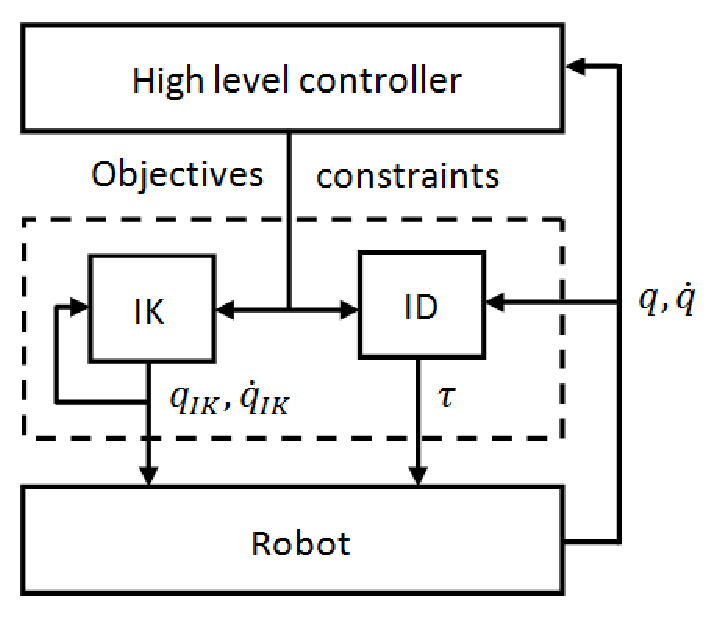
\includegraphics[width=0.3\textwidth]{images/sys.eps}}
    \caption{
      The task dependent high level controller generates a set of desired 
      objectives such as CoM or limb motion, and constraints such as CoP and 
      joint limits. The proposed full body controller, which is contained by
      the dashed rectangle, takes the high level objectives and robot states 
      $(q,\dot{q})$ as inputs and outputs position $q_{IK}$, velocity 
      $\dot{q}_{IK}$ and torque $\tau$ for each joint, which are used as 
      desired values, $q_d, \dot{q}_d$ and $\tau_d$, in \eref{eq:servo}. Note that IK uses its 
      own internal states rather than the measured robot states. 
      }\label{fig:sys} 
  \end{center}
\end{figure}  
 
On our Atlas robot, a 28 degrees of freedom hydraulic robot built by Boston 
Dynamics, joint level servos compute valve commands based on 
\begin{equation}
  i = K_p(q_d-q) + K_d(\dot{q}_d-\dot{q}) + K_f(\tau_d-\tau) + c,
  \label{eq:servo}
\end{equation}
where $q_d, \dot{q}_d, \tau_d$ are desired joint position, velocity and torque,
$q, \dot{q}, \tau$ are measured, and 
$c$ contains the constant valve bias term plus some other auxiliary feedback
and feedforward terms. 
The joint level servos run at 1$kHz$, while $q_d,\dot{q}_d$ and $\tau_d$ can be
updated at the same frequency.  
In previous work \cite{stephens_thesis,whitman_thesis,sfeng_online}, 
we focused on torque control with ID that computes $\tau_d$. 
To take full advantage of the on-board high bandwidth PD servo, we need to 
generate reference $q_d$ and $\dot{q}_d$. 

Using full body inverse dynamics for force control has become a popular topic
in recent humanoid research. Much of the research originates from the 
operational space formulation \cite{khatib_op_space_ctrl}. 
Within this broad category, reference motions in task space are specified, 
and convex optimization is used to handle constraints and solve for controls
that best track the reference motions. 
Although detailed formulations differ, most active research has converged to 
formulating the floating base inverse dynamics as a QP problem. 
Hierarchical approaches \cite{eth_id,Hutter01052014,alex_hir,saab_fast_hir_qp,deLasa_hir,wensing_hir,sentis_wbc}
are used to resolve redundant degrees of freedom in humanoid robots. 
These approaches typically ensure low priority objectives are within the null
space of higher priority ones. 
We prefer using soft costs as opposed to hard constraints for better numerical 
stability especially in situations where no feasible solutions exist for the 
specified objectives.
There is also much interest in formulating a smaller QP problem to reduce 
computation time. Contact wrenches can be removed from the
equations of motion using orthogonal decomposition \cite{usc_id1}.
Ott et al. \cite{ott_force_alloc} use simple PD servos to generate a 
desired net ground reaction wrench, which is then distributed among predefined 
contacts using optimization.
Ramos et al. \cite{ramos_dyn_walking} solve a smaller QP with decoupled dynamics. 
Lee et al. \cite{lee_separate_grf} present a two level optimization setup. 
The first level optimizes individual ground reaction wrenches and center of pressure
(CoP) for each contact and the resulting admissible change in centroidal momenta. 
Then another least square problem is solved for the state acceleration. 
Joint torques are generated explicitly. 
Koolen et al. \cite{ihmc_vrc} generate desired centroidal momenta change based 
on instantaneous capture point, and uses QP to optimize for acceleration and 
contact wrenches. Joint torques are then generated with explicit inverse dynamics. 
A novel QP solver is implemented by Kuindersma et al. \cite{scott_qp} to exploit
the observation that inequality constraints rarely change in this context.

During the DRC Trials, we continued to use the same approach to ID that was 
previously developed in our group \cite{stephens_thesis,whitman_thesis,sfeng_online} 
that is similar to the work by de Lasa et al. \cite{deLasa_hir} and 
Bouyarmane et al. \cite{bouyarmane_vrc} 
We optimized for acceleration, torque, and contact wrenches simultaneously 
on the full robot model. This design choice was intuitive, and gave us the
most flexibility in terms of trading off directly among physical quantities
of interest. Recently, we remove the explicit dependency on joint torques in
ID using the decoupling presented by Herzog, et al. \cite{alex_hir} to speed
up computation.
%It also provides an easy way to properly manage all constraints on 
%contact wrenches and joint torques. It does result in a bigger QP problem, 
%but is still solvable in real time with a standard QP solver. 

ID does not generate $q_d$ or $\dot{q}_d$ directly for \eref{eq:servo}.
For the DRC Trials, we introduced a separate inverse kinematics (IK) controller to
explicitly compute these kinematic references. 
For more dynamic behaviors, our recent work prefers integrating the acceleration
computed by ID into desired velocity that properly obeys dynamic constraints.  
Similar to ID, our IK was also formulated as a QP, where the unknowns are the 
generalized velocities, $\dot{q}$, of the floating base and all the joints. 
At each time step, we solved for $\dot{q}$ that obeyed kinematic constraints 
and minimized a combination of costs. $q$ was computed by integrating $\dot{q}$. 
Our IK approach was similar in spirit to the work by Mistry et al.\cite{mistry_ik} 
Solving for $\dot{q}$ and integrating to obtain $q$ was the primary difference
between our approach and most traditional IK approaches \cite{kajita03,asimo}. 
The incremental method can get stuck in local minima, but faster computation
is more suitable for real time control purposes. 
This formulation also fitted nicely with the tel-operation heavy paradigm we 
adopted for the DRC Trials. 

The main contribution of this work is the successful application to a physical 
system and many modifications of existing techniques, as well as 
the lessons learned and intellectual challenges from this effort. 
The remainder of this paper is arranged as follows. 
\sref{sec:fbc} provides a brief description of the common formulation for 
our ID and IK controller, which are then detailed in \sref{sec:ID} and \sref{sec:IK}
respectively.
Three applications are shown in \sref{sec:trials_tasks} 
in the context of the DARPA Robotics Challenge Trials that took place in 
December 2013. 
A brief overview of recent work in progress that aims at faster walking 
is presented in \sref{sec:new_stuff}.
Finally, discussions and conclusions are provided 
in \sref{sec:dis} and \sref{sec:conclusion}.

%%%%%%%%%%%%%%%%%%%%%%%%%%%%%%%%%%%%%%%%%%%%%%%%%%%%%%%%%%%%%%%%%%%%%%%%%%%%%%%%

\section{Full body control}
\label{sec:fbc}
For many tasks, we specify desired Cartesian motions for specific locations on 
the robot (e.g. foot, hand and CoM) in the high level controller. 
The proposed low level controller takes these as inputs, and computes physical 
quantities for each individual joint such as joint position, velocity and torque. 
These outputs are then used as references in the joint
level servos on the robot. \fref{fig:sys} shows a block diagram for the overall 
system. Joint position and velocity are computed separately 
from joint acceleration and torque. We refer to the former problem as inverse 
kinematics (IK) and the latter as inverse dynamics (ID). Both are formulated as 
Quadratic Programming (QP) problems. 
\begin{equation}
  \begin{split}
  \min_{\QPx}\;\; & 0.5\QPx^TG\QPx + g^T\QPx \\
  s.t.\;\; & C_E\QPx + c_E = 0 \\
  & C_I\QPx + c_I \geq 0.
  \end{split}
	\label{eq:qp}
\end{equation} 
The unknown, ${\QPx}$, and constraints, $C_E, c_E, C_I$ and $c_I$, are problem specific,
which we will elaborate on in the following sections. Both QP problems are solved at 
each time step in a 3$ms$ control loop with a standard solver. 

For both problems, we optimize a cost function of the form $0.5\|A\QPx-b\|^2$. 
Thus $G = A^TA$, and $g = -A^Tb$ in \eref{eq:qp}.
$A$ and $b$ can be decomposed into smaller blocks as 
\begin{equation}
  A = \begin{bmatrix} w_0A_1 \\ w_1 A_1 \\ \vdots \\ w_nA_n \end{bmatrix},
  b = \begin{bmatrix} w_0b_0 \\ w_1 b_1 \\ \vdots \\ w_nb_n \end{bmatrix}.
  \label{eq:cost}
\end{equation}
Each row emphasizes a certain desired behavior with weight, $w_i$.

\section{Inverse dynamics}
\label{sec:ID}
The equations of motion and the constraint equations for a floating base humanoid 
robot can be described as
\begin{equation}
  \begin{split}
    M(q)\ddot{q} + h(q,\dot{q}) &= S\tau + J^T(q)\lambda \\
    J(q)\ddot{q} + \dot{J}(q,\dot{q})\dot{q} &= \ddot{x},
  \end{split}
\end{equation}
where $(q,\dot{q})$ is the full state of the system including a six DoF floating 
base, $M(q)$ is the inertia matrix, $h(q,\dot{q})$ 
is the sum of gravitational, centrifugal and Coriolis forces, $S$ is a selection
matrix, where the first six rows that correspond to the six DoF floating base are 
zeros, and the rest form an identity matrix, $\tau$ is a vector of joint torques, 
$J^T(q)$ is the Jacobian matrix for all the contacts, $\lambda$ is a vector
of all contact wrenches in the world frame, and $x$ is a vector of  
contact position and orientation in Cartesian space. $\lambda$ and $J^T$'s 
dimensions depend on the number of contacts. 

We can rewrite the equations of motion as 
\begin{equation}
  \begin{bmatrix} M(q) & -S & -J^T(q) \end{bmatrix} 
  \begin{bmatrix} \ddot{q} \\ \tau \\ \lambda \end{bmatrix}
  +h(q,\dot{q}) = 0.
		\label{eq:eom}
\end{equation}
Given a state, $(q,\dot{q})$, the equations of motion are linear in terms of 
$\begin{bmatrix} \ddot{q} & \tau & \lambda \end{bmatrix}^T$. 

For ID, $\QPx = \begin{bmatrix} \ddot{q} & \tau & \lambda \end{bmatrix}^T$.
\eref{eq:eom} is enforced as equality constraints. The 
inequality constraints consist of joint torque limits, contact force limits 
due to friction cone constraints, and contact torque limits due to center of 
pressure (CoP) remaining in the support polygon. 

\subsection{Cost function}
We list a few examples of the objectives that can be plugged into the rows of
\eref{eq:cost}. 
\subsubsection{Cartesian space acceleration} 
Since
\begin{equation}
  \ddot{x} = J(q)\ddot{q} + \dot{J}(q,\dot{q})\dot{q},
\end{equation}
we can penalize deviation from the desired Cartesian acceleration using
\begin{equation}
  \begin{split}
    A_{cart} &= \begin{bmatrix} J(q) & 0 & 0 \end{bmatrix} \\
    b_{cart} &= \ddot{x}^* -\dot{J}(q,\dot{q})\dot{q}.
		\label{eq:id_cart}
  \end{split}
\end{equation}  
The input $\ddot{x}^*$ is computed by
\begin{equation}
  \ddot{x}^* = K_p(x^*_d - x) + K_d(\dot{x}^*_d - \dot{x})  + \ddot{x}_d^*,
	\label{eq:id_cart_pd}
\end{equation}
where $x^*_d$, $\dot{x}^*_d$ and $\ddot{x}_d^*$ are specified by a higher 
level controller, and $x$ and $\dot{x}$ are computed by forward kinematics 
based on the estimated current robot state. 
Many objectives such as CoM, hand, foot and torso motions are 
specified with this form. Depending on the tasks, we sometimes drop the
rows in \eref{eq:id_cart} that we do not want to track. 

Rather than treating contacts as hard constraints, we find that using a soft 
penalty with a high weight is generally more numerically stable.
For such contact costs, we set $\ddot{x}^* = 0$ in \eref{eq:id_cart_pd}.

%\subsubsection{Net external force and center of mass motion}
%The relationship between CoM linear acceleration and net external force is 
%\begin{equation*}
%  F_{lin} = m(\ddot{x}_{com}+\begin{bmatrix} 0 & 0 & g \end{bmatrix}^T),
%\end{equation*}
%where $m$ is the total mass, and $g$ is the gravitational acceleration.
%Net torque and change in angular momentum $\dot{L}$ are related in a similar way
%\begin{equation*}
%  F_{ang} + (x_{contact}-x_{com}) \times F_{lin} = I\dot{\omega}_{com},
%\end{equation*} 
%where $I$ is the total moment of inertia, and $\dot{\omega}_{com}$ is the 
%angular acceleration. We can compute
%\begin{equation*}
%  \begin{split}
%    A_{comF} &= \begin{bmatrix} 0 & 0 & \begin{bmatrix} I_{3 \times 3} & 0\end{bmatrix} \end{bmatrix} \\
%    b_{comF} &= m(\ddot{x}_{com}^*+\begin{bmatrix} 0 & 0 & g \end{bmatrix}^T)
%  \end{split}
%\end{equation*}
%and
%\begin{equation*}
%  \begin{split}
%    A_{comTau} &= \begin{bmatrix} 0 & 0 & \begin{bmatrix} Cross(x_{contact},x_{com}) & I_{3 \times 3} \end{bmatrix} \end{bmatrix} \\
%    b_{comTau} &= I\dot{\omega}_{com}^*.
%  \end{split}
%\end{equation*}
%$I_{3 \times 3}$ is a 3 by 3 identity matrix. $\ddot{x}_{com}^*$ and 
%$\dot{\omega}_{com}^*$ are desired linear and angular accelerations. 
%$Cross(x_{contact},x_{com})$ is the matrix representing a cross product between
%$(x_{contact}-x_{com})$ and $F_{lin}$.

\subsubsection{Center of pressure tracking} 
CoP in the foot frame is
\begin{equation}
  p = \begin{bmatrix} -^{b}M_{y} / ^{b}F_{z} \\ ^{b}M_{x} / ^{b}F_{z} \end{bmatrix},
\end{equation}
where $^{b}M$ and $^{b}F$ are contact forces and torques in the foot frame.
We can penalize CoP deviation with
\begin{equation}
  \begin{split}
    A_{cop} &= \begin{bmatrix} 0 & 0 & \begin{bmatrix} 0 & 0 & p_x^* & 0 & 1 & 0 \\ 0 & 0 & p_y^* & -1 & 0 & 0 \end{bmatrix} \begin{bmatrix} R & 0 \\ 0 & R \end{bmatrix} \end{bmatrix} \\
    b_{cop} &= 0,
  \end{split}
\end{equation}
where $(p_x^*, p_y^*)$ is the desired CoP in the foot frame given by
a high level controller, and $R$ is the rotation matrix from the world frame to
the foot frame.

\subsubsection{Weight distribution} 
In double support, we specify a desired weight distribution by  
$w^* = F_{zl} / (F_{zl}+F_{zr})$, where $F_{zl}$ and $F_{zr}$ are the vertical 
forces at the left and right foot. We add this term to the cost function with
\begin{equation}
  \begin{split}
    A_{weigt} &= \begin{bmatrix} 0 & 0 & S_{weight} \end{bmatrix} \\
    b_{weigt} &= 0.
  \end{split}
\end{equation}
$S_{weight}$ is a row vector with zeros, except $S_{weight}(i_{F_{zl}}) = 1-w^*$ and 
$S_{weight}(i_{F_{zr}}) = -w^*$, where $i_{F_{zl}}$ and $i_{F_{zr}}$ are indices correspond
to $F_{zl}$ and $F_{zr}$.

\subsubsection{Direct tracking and regularization} 
We can also directly penalize $\QPx$ from desired values with
\begin{equation}
  \begin{split}
    A_{state} &= W \\
    b_{state} &= \begin{bmatrix} \ddot{q}^* & \tau^* & \lambda^* \end{bmatrix}^T,
  \end{split}
	\label{eq:id_reg}
\end{equation}
where $W$ is a diagonal weighting matrix. 
Zero is used if no target value is specified except for the vertical forces, which 
are regularized using gravitational forces. This term is useful for directly 
controlling specific joints or contact wrenches. It also regularizes $\QPx$ to make the
QP problem well conditioned.

\subsubsection{Change in torques} 
To avoid high frequency oscillations in torque commands, we penalize changes in 
$\tau$ with
\begin{equation}
  \begin{split}
    A_{d\tau} &= \begin{bmatrix} 0 & I & 0 \end{bmatrix} \\
    b_{d\tau} &= \tau_{prev},
  \end{split}
\end{equation} 
where $\tau_{prev}$ is from the last time step.

%Weights are summarized in \tref{tab:QPparam}. $w_{qdd}$ is for joint acceleration. 
%$w_{com}$ and $w_{utorsowd}$ are for CoM position acceleration and upper torso
%orientation acceleration. $w_{footdd}$ is for foot position and orientation acceleration. 
%$w_{comF}$ and $w_{comTau}$ are for net external force and torque. $w_{regF}$ and 
%$w_{regTau}$ are regularization weights for contact force and joint torques. $w_w$ is 
%for weight distribution. $w_{cop}$
%is for center of pressure. $w_{Fd}$ and $w_{Taud}$ penalize changes in contact
%force and joint torques between two consecutive time steps. 

\subsection{Constraints} 
\eref{eq:eom} is used as equality constraints. Torque limits can be 
easily added into the inequality constraints. Friction constraints are 
approximated by
\begin{equation}
  \begin{split}
    | ^bF_x | &\leq \mu ^bF_z \\
    | ^bF_y | &\leq \mu ^bF_z. 
  \end{split}
\end{equation}
The forces and torques at the feet need to obey CoP constraints,
%Ankle torques are limited by the normal forces and foot size, which can be written as
\begin{equation}
  \begin{split}
    d_x^- &\leq -^{b}M_{y} / ^{b}F_{z}  \leq d_x^+ \\
    d_y^- &\leq ^{b}M_{x} / ^{b}F_{z}  \leq d_y^+,
  \end{split}
	\label{eq:id_cop_con}
\end{equation} 
where $^{b}F$ and $^{b}M$ denote forces and torques in the foot frame, and 
$d^-$ and $d^+$ are the sizes of foot. The body frame forces and torques are 
computed by rotating $\lambda$ into the foot frame. 

%%%%%%%%%%%%%%%%%%%%%%%%%%%%%%%%%%%%%%%%%%%%%%%%%%%%%%%%%%%%%%%%%%%%%%%%%%%%%%%%   
\section{Inverse kinematics}
\label{sec:IK}
Unlike traditional IK approaches that generate positions for the entire desired 
trajectory ahead of time, we compute velocities at each time step and integrate 
them to get positions. The controller can be more responsive to changes in 
the high level commands, and computation is averaged across the course of motion. 

For the IK QP, $\QPx = \dot{q}$, and the numerically integrated floating base 
position and joint position is denoted by $q_{ik}$. Our IK formulation is very 
similar to ID's except that the internal states are used for forward kinematics 
and generating target velocities. 
Separate internal states within IK are necessary to accumulate previous 
correctional velocities. This can lead to divergence between IK's internal 
state and the state estimator's, particularly the root position. 
Resetting IK's state to match the state estimator's is one option, 
but it introduces sudden discrete changes. 
We use ''anchor'' points instead, which is detailed in \sref{sec:anchor}.
The internal states are set to the real robot states in the 
initialization stage. All the internal states are denoted with subscripts $_{ik}$. 

\subsection{Cost function}
We list a few examples of the objectives that can be plugged into 
\eref{eq:cost}. 
\subsubsection{Cartesian space velocity} 
We penalize deviation from the desired Cartesian velocity, $\dot{x}^*$, with 
\begin{equation}
  \begin{split}
    A_{cart} &= J(q_{ik}) \\
    b_{cart} &= \dot{x}^*,
  \label{eq:ik_cart}
  \end{split}
\end{equation}
where 
\begin{equation}
  \dot{x}^* = K_p(x^*_d - x_{ik}) + \dot{x}^*_d.
  \label{eq:ik_cart_pd}
\end{equation}
We use a different set of $K_p$ here than in ID. 
Cartesian space tracking and contacts are both handled with 
\eref{eq:ik_cart} and \eref{eq:ik_cart_pd}. Although the weights and desired 
targets, $x^*_d$ and $\dot{x}^*_d$ are different.

\subsubsection{Direct tracking and regularization} 
\begin{equation}
  \begin{split}
    A_{state} &= W \\
    b_{state} &= \dot{q}^*,
  \end{split}
	\label{eq:ik_reg}
\end{equation} 
where $W$ is a diagonal weighting matrix, 
and $\dot{q}^*$ can be target joint velocity or 0 for regularization.

\subsubsection{Change in velocity} 
\begin{equation}
  \begin{split}
    A_{d\dot{q}} &= I \\
    b_{d\dot{q}} &= \dot{q}_{prev},
  \end{split}
\end{equation} 
where $\dot{q}_{prev}$ is the result from the previous time step. This 
term is useful to eliminate high frequency oscillation in the generalized 
velocities. 

\subsection{Constraints}
We do not impose equality constraints in the IK QP. Inequality constraints 
mainly consist of joint limits. Depending on the application, we also add 
constraints in Cartesian space. 
%For manipulation, we constrain the CoM to 
%be within the support polygon. For the ladder task in DRC, we constrain the 
%elbows to be within the railings on the ladder. 

The joint limit constraints are 
\begin{equation}
  q^- \leq q_{ik} + \dot{q}dt \leq q^+,
\end{equation}
where $dt$ is the time step, and $q^-$ and $q^+$ are the upper and lower joint 
limit. 
For Cartesian space position constraints, 
\begin{equation}
  x^- \leq x_{ik} + J(q_{ik})\dot{q}dt \leq x^+,
	\label{eq:ik_cart_ineq}
\end{equation}
where $x^-$ and $x^+$ are the upper and lower limits. 
Velocity constraints in joint space can be easily added, and Cartesian space 
velocity constraints need to be transformed by a Jacobian matrix. 
 
\subsection{Anchor points}
\label{sec:anchor}
Unlike ID, where we demand zero acceleration for the contacts,
we introduce desired position targets in IK, which we refer to as anchor points. 
Since IK only relies on its internal states, without any external feedback, 
the internal states will diverge from the state estimator's.
For example, suppose we wish to take a step of some specific length. 
The IK controller will hit the desired foot step almost perfectly if not 
violating any constraints. The real robot will not due to tracking errors.
After taking several steps, the IK controller will end up in a significantly
different location than the state estimator. 
Because the high level controllers generate desired Cartesian targets 
based on the state estimator, we need to compensate for this 
divergence within the IK controller. 
In order to tie IK's internal states to the state estimator's, we specify a Cartesian
target, $x_{anchor}^*$, that slowly tracks the estimated contact
pose, $x_{contact}$.
\begin{equation}
\label{eq:leaky}
  x_{anchor}^* = \alpha x_{contact} + (1-\alpha)x_{anchor}^*.
\end{equation}
In \eref{eq:ik_cart_pd}, $x_{anchor}^*$ replaces $x^*_d$, and $\dot{x}^*_d = 0$.
$\alpha = 0.005$ for static walking. 
$x_{anchor}^*$ is initialized to IK's internal value upon establishing the contact. 
Since $x_{anchor}^*$ contains all the information about long term tracking error
and state estimator drift, and IK tracks $x_{anchor}^*$ well, we can use 
$x_{anchor}^*$ to update IK's internal states to match the state estimator's. ID is 
not affected since target contact acceleration is always set to zero in \eref{eq:id_cart_pd}.
 
%%%%%%%%%%%%%%%%%%%%%%%%%%%%%%%%%%%%%%%%%%%%%%%%%%%%%%%%%%%%%%%%%%%%%%%%%%%%%%%%
\section{Applications}
\label{sec:trials_tasks}
The proposed full body controller has been tested on Boston Dynamics's Atlas robot,
which has 28 hydraulic actuators, six for each leg and arm, three for the back 
joints, and one for neck pitch. 
The controller was used for the rough terrain walking, ladder climbing
and manipulation tasks in the DARPA Robotics Challenge Trials in December 2013. 
For all three applications, the state estimator was based on the work of 
Xinjilefu et al. \cite{xinji}

\subsection{Static walking}
\label{sec:static_walking}
For the DRC Trials, we used a simple static walking strategy. 
Desired CoM motion was represented with a quintic spline. 
Swing foot trajectory was generated with piecewise splines. 
\fref{fig:terrain_pic} shows snapshots of the Atlas robot traversing piled cinder
blocks with tilted tops, and CoM and feet trajectories are plotted in 
\fref{fig:walk_com}. 
The desired CoP trajectory was generated using a Linear Inverted Pendulum 
Model (LIPM). 
\fref{fig:walk_cop} shows CoP tracking for the Atlas robot stepping up piled cinder blocks. 

Most other teams at the DRC Trials built a map with laser point clouds and 
selected foot steps with either a human operator or some combination of 
heuristics and simple planning. 
Due to forward kinematic errors in the robot, registering laser points while
moving did not work well. 
The robot had to be stationary to generate high fidelity maps. 
To avoid extensive periods of standing still, we provided our human operator 
with a live camera stream augmented with the current swing foot pose computed
from forward kinematics, and let the operator ``nudge'' the swing foot around
in Cartesian space by commanding offsets in desired foot position and orientation. 
Once the operator was satisfied with the foot pose, a ``continue'' command was 
issued, the robot put the swing foot straight down until ground contact. 
On the downside, our approach required more (and more difficult) inputs from 
the operator, and had much longer single support phase when the operator 
commands were being issued.

The following modifications to the full body controller as described above were
made for the walking task:
\subsubsection{Ankle torque controlled}
For better CoP control, the stance ankles were controlled in pure torque mode. 
IK solutions for the stance ankle joints were ignored. 
The downside was that the ankle position errors propagated up the kinematic 
chain, and resulted in errors in swing foot tracking. 
An integrator on the desired swing foot position was used to compensate for this. 
\begin{equation}
  \label{eq:int}
  \begin{split}
    err_{swing} &= err_{swing} + K_i(x_{swing_d}' - x_{swing}) \\
    x_{swing_d}^* &= x_{swing_d}' + err_{swing},
  \end{split}
\end{equation}  
where $x_{swing_d}'$ is the desired swing foot position from the operator or a 
foot step planner, 
$x_{swing}$ is the computed position from forward kinematics, 
and $x_{swing_d}^*$ is used as inputs in \eref{eq:id_cart_pd} and 
\eref{eq:ik_cart_pd}. 

\subsubsection{Toe-off}
For static walking, the CoM needs to be completely shifted to the next stance foot 
during double support. 
When taking longer strides or stepping to a greater height, extending the 
rear leg knee alone is often insufficient to move the CoM all the way. 
Toe-off is one solution to this problem. 
During double support, toe-off was triggered when the rear knee approached the 
joint angle limit (straight knee). 
During toe-off, we shifted the rear foot reference point, where the Jacobian was 
computed, to the toe. 
The contact cost terms in \eref{eq:id_cart} and \eref{eq:ik_cart} for the rear 
foot were modified. 
Position terms remained the same. 
For the rotational terms, we first computed
\begin{equation}
  \begin{split}
    A^{ID}_{rot} &= \begin{bmatrix} R^T J_{rot}(q) & 0 & 0 \end{bmatrix} \\
		b^{ID}_{rot} &= R^T (\ddot{x}^*_{rot} - \dot{J}_{rot}(q,\dot{q}) \dot{q}) \\
    A^{IK}_{rot} &= R^T J_{rot}(q_{ik}) \\
    b^{IK}_{rot} &= R^T \dot{x}^*_{rot} \\
  \end{split}
	\label{eq:cart_rot}
\end{equation}   
for ID and IK respectively, where $R$ is the orientation of the foot. 
Only the first and third rows in \eref{eq:cart_rot}, that correspond to 
roll and yaw motion were added to the cost functions.
$\ddot{x}^*_{rot}$ was set to zero, and $\dot{x}^*_{rot}$ was computed with \eref{eq:leaky}.
We also set $d^-_y = d^+_y = 0$ in \eref{eq:id_cop_con}. 
This effectively turned the rear foot contact into an unactuated pin joint 
around the pitch axis. 
A slightly bent rear knee angle was given as desired in \eref{eq:id_reg} and 
\eref{eq:ik_reg} as well.

\subsubsection{Integrator for desired CoM offset}
\label{sec:com_int}
Assuming the robot is moving slowly enough, we approximated the true CoM 
with the measured CoP, and computed $CoM_{err} = CoP - CoM_{model}$.
During the second half of double support and single support phase, 
we integrated $CoM_{err}$ to offset the desired CoM so that the true CoM was at 
the middle of the supporting foot. 
The integrator was set up similarly to \eref{eq:int}. 

\begin{figure}
  \begin{center}
    {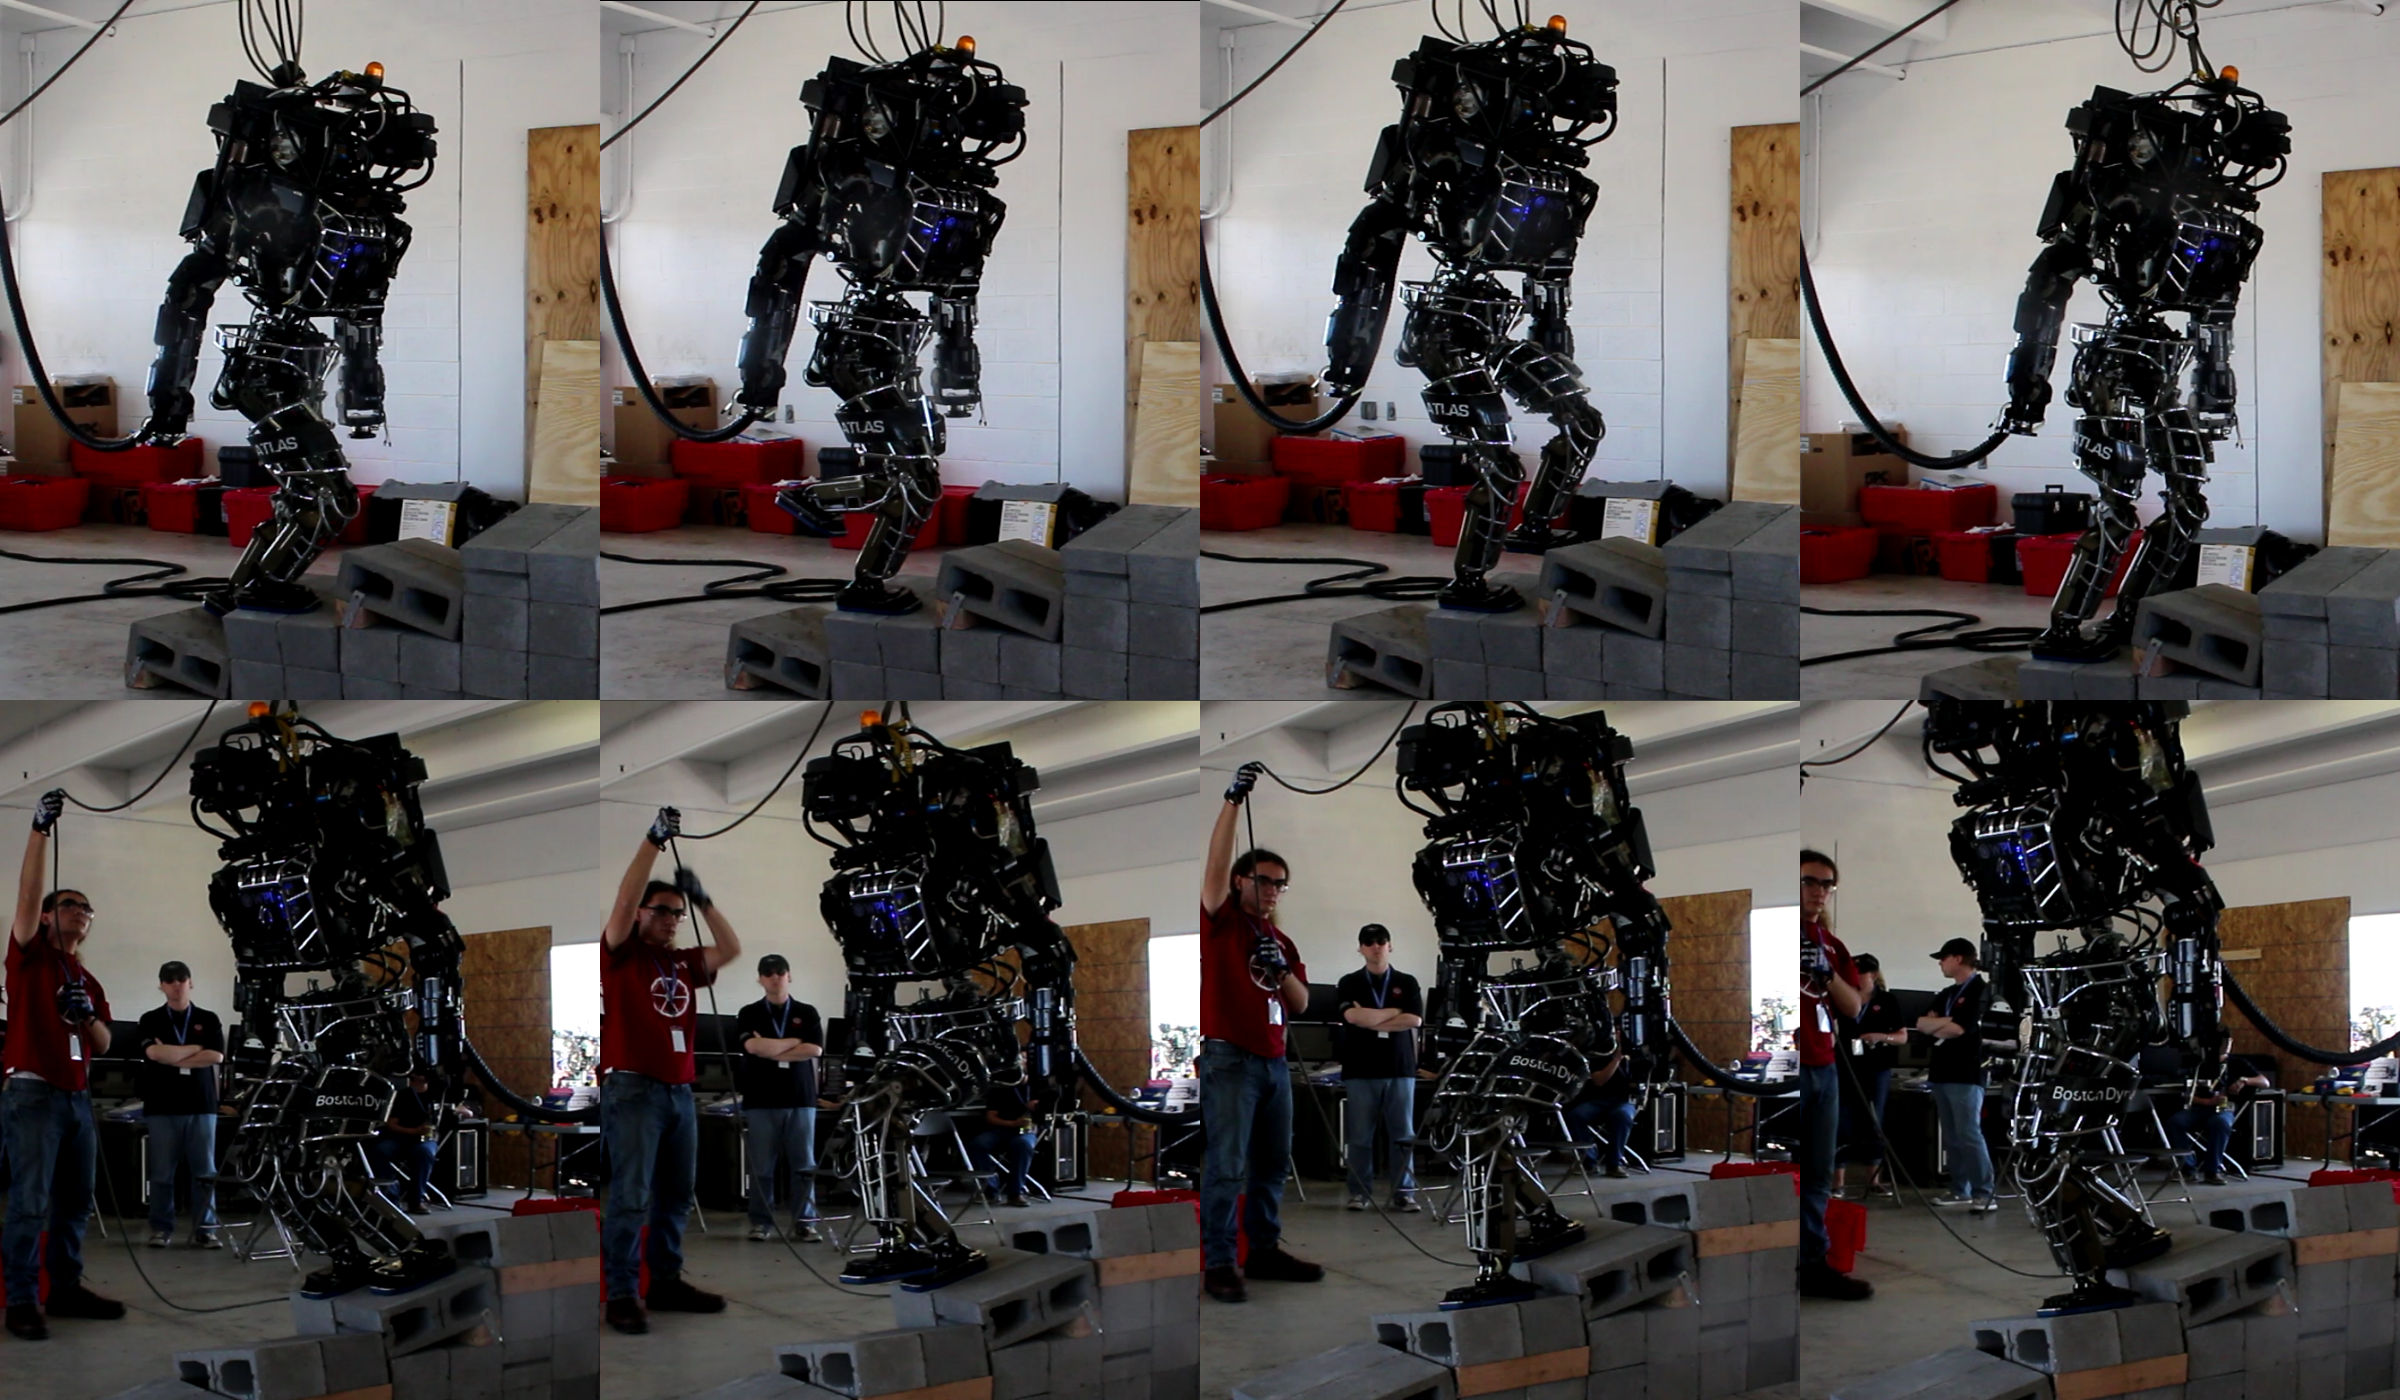
\includegraphics[width=1\textwidth]{images/terrain.eps}}
    \caption{
      These photos show the Atlas robot practicing for the third segment of the 
      terrain task for the DRC Trials. The snapshots were taken every 5 seconds.
      }\label{fig:terrain_pic} 
  \end{center}
\end{figure}

%TODO
% UPDATE FIGURES
\begin{figure}
  \begin{center}
    \subfigure[Measured feet and CoM trajectories in $XY$ plane for terrain task]
      {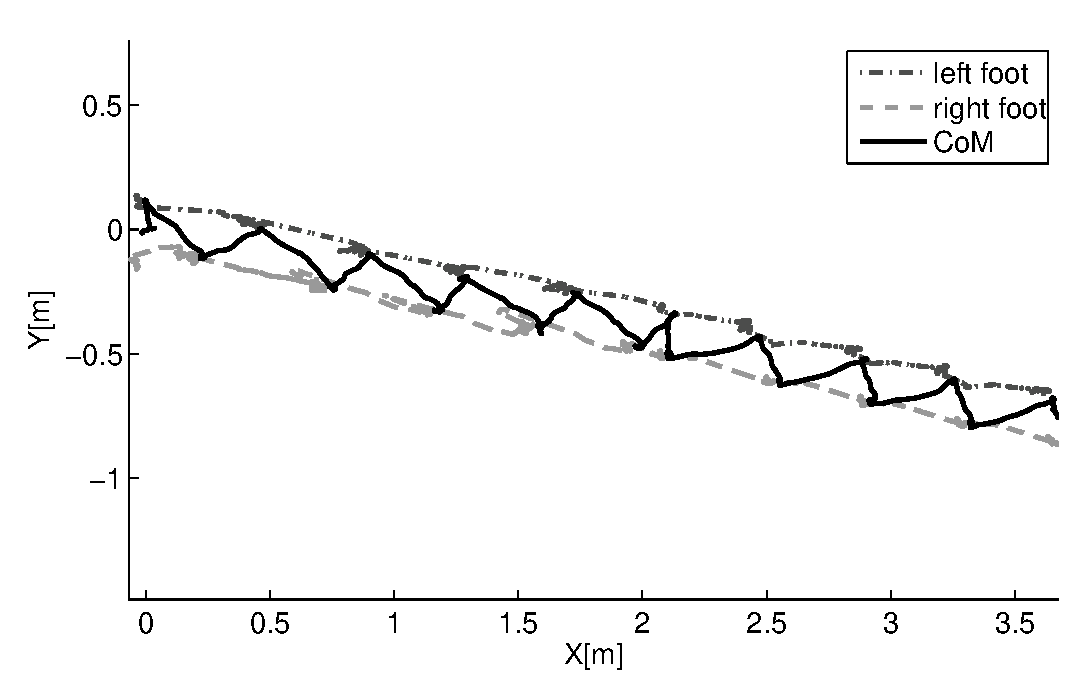
\includegraphics[width=0.48\textwidth]{images/walking_xy_gray.eps} \label{subfig:walking_xy}}
    \subfigure[Measured feet and CoM trajectories in $XZ$ plane for terrain task]
      {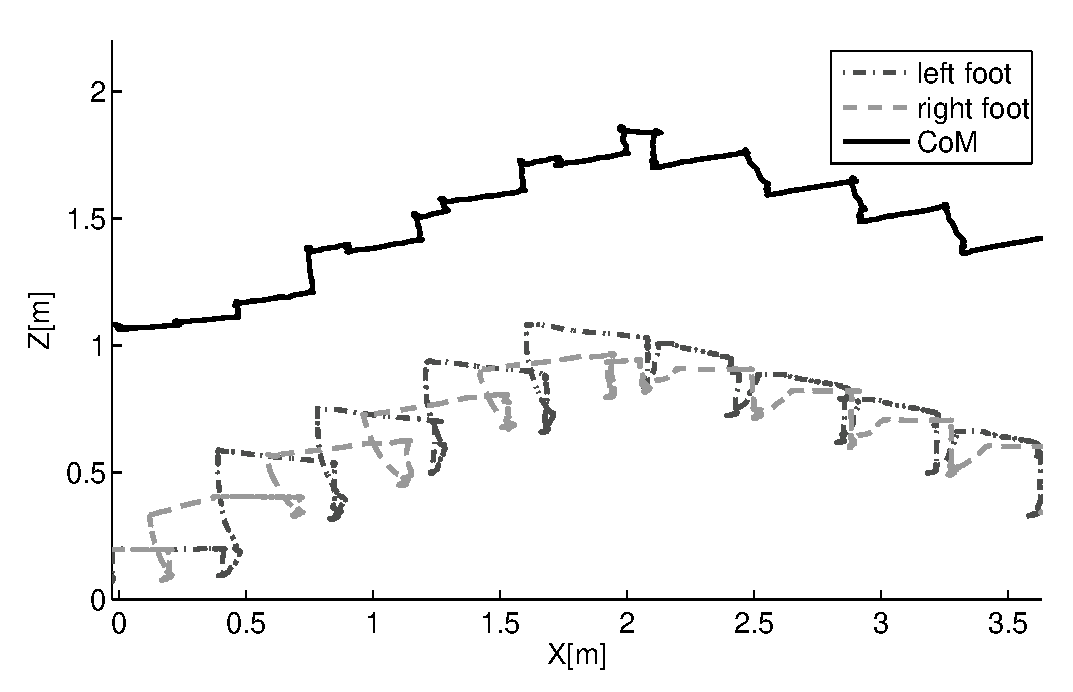
\includegraphics[width=0.48\textwidth]{images/walking_xz_gray.eps} \label{subfig:walking_xz}} 
    \caption{                    
      These plots show the Atlas robot traversing the third segment of the terrain 
      task. 
      $X$ axis is the forward direction, $Y$ points to the robot's left, and
      $Z$ points upward. 
      The robot walked in a straight line in reality. 
			Without external observation, our state estimator drifted significantly.
			}\label{fig:walk_com} 
  \end{center}
\end{figure}     

%TODO
\begin{figure}
  \begin{center}
    %\subfigure[CoP in X axis]
      %{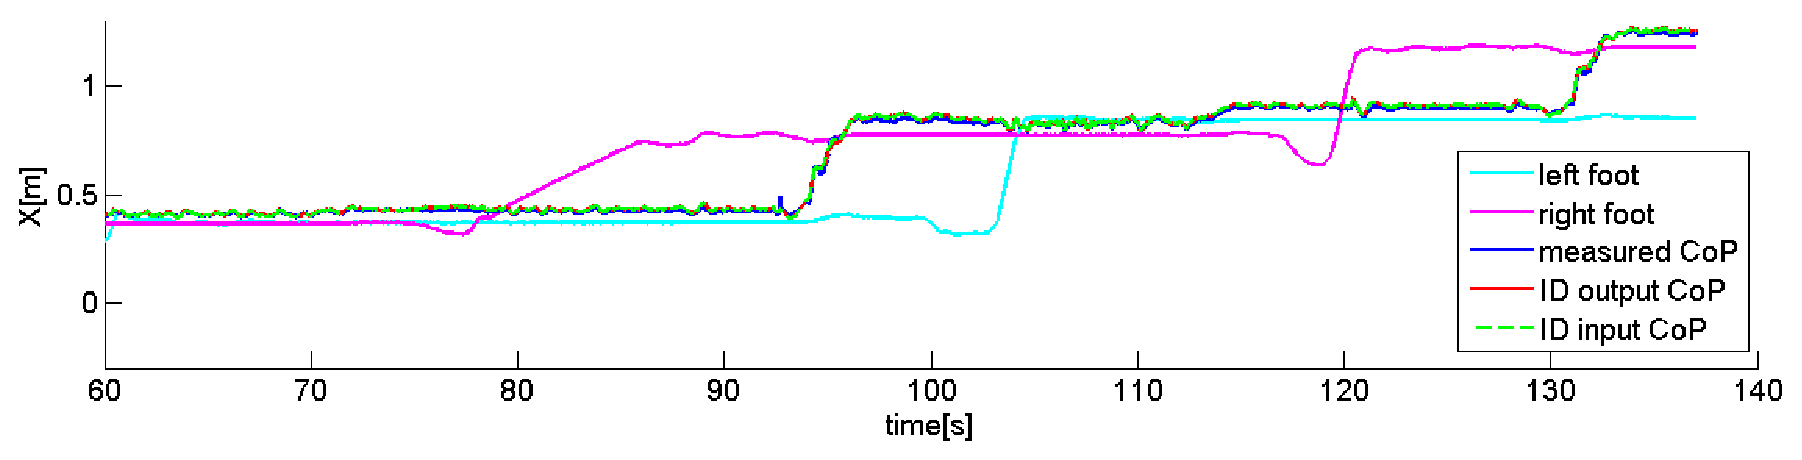
\includegraphics[width=.45\textwidth]{images/cop_x.eps} \label{subfig:atlas_cop_x}}
    %\subfigure[CoP in Y axis]
      %{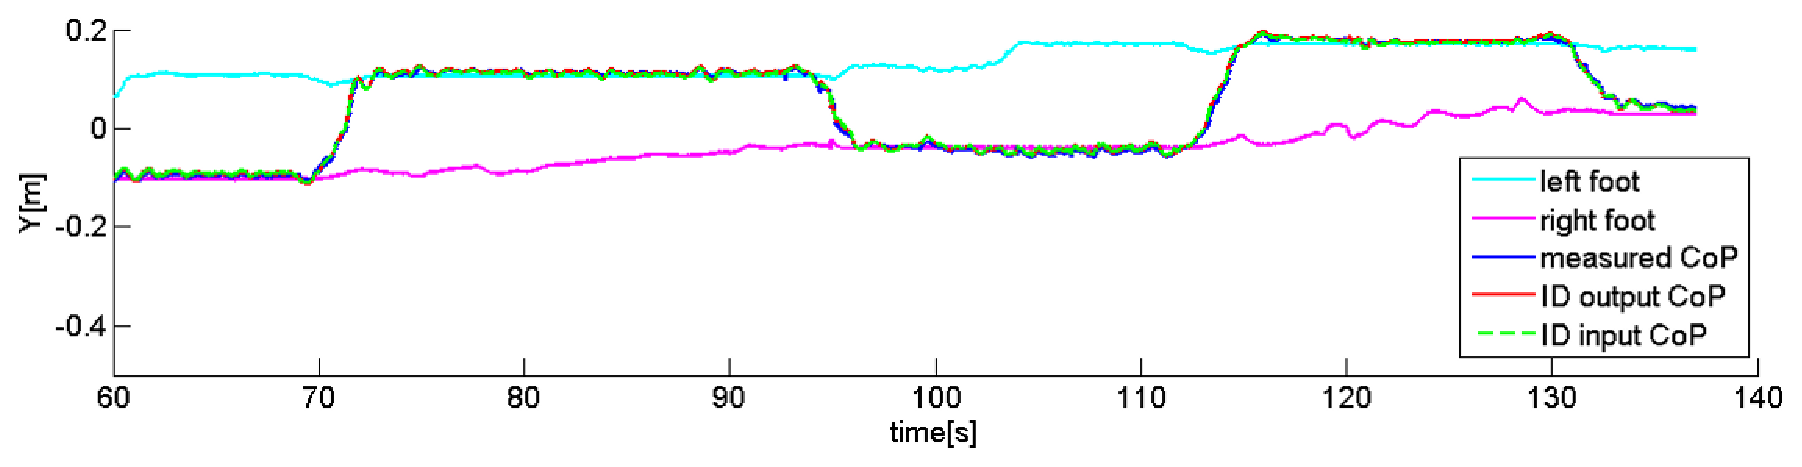
\includegraphics[width=0.45\textwidth]{images/cop_y.eps} \label{subfig:atlas_cop_y}}
    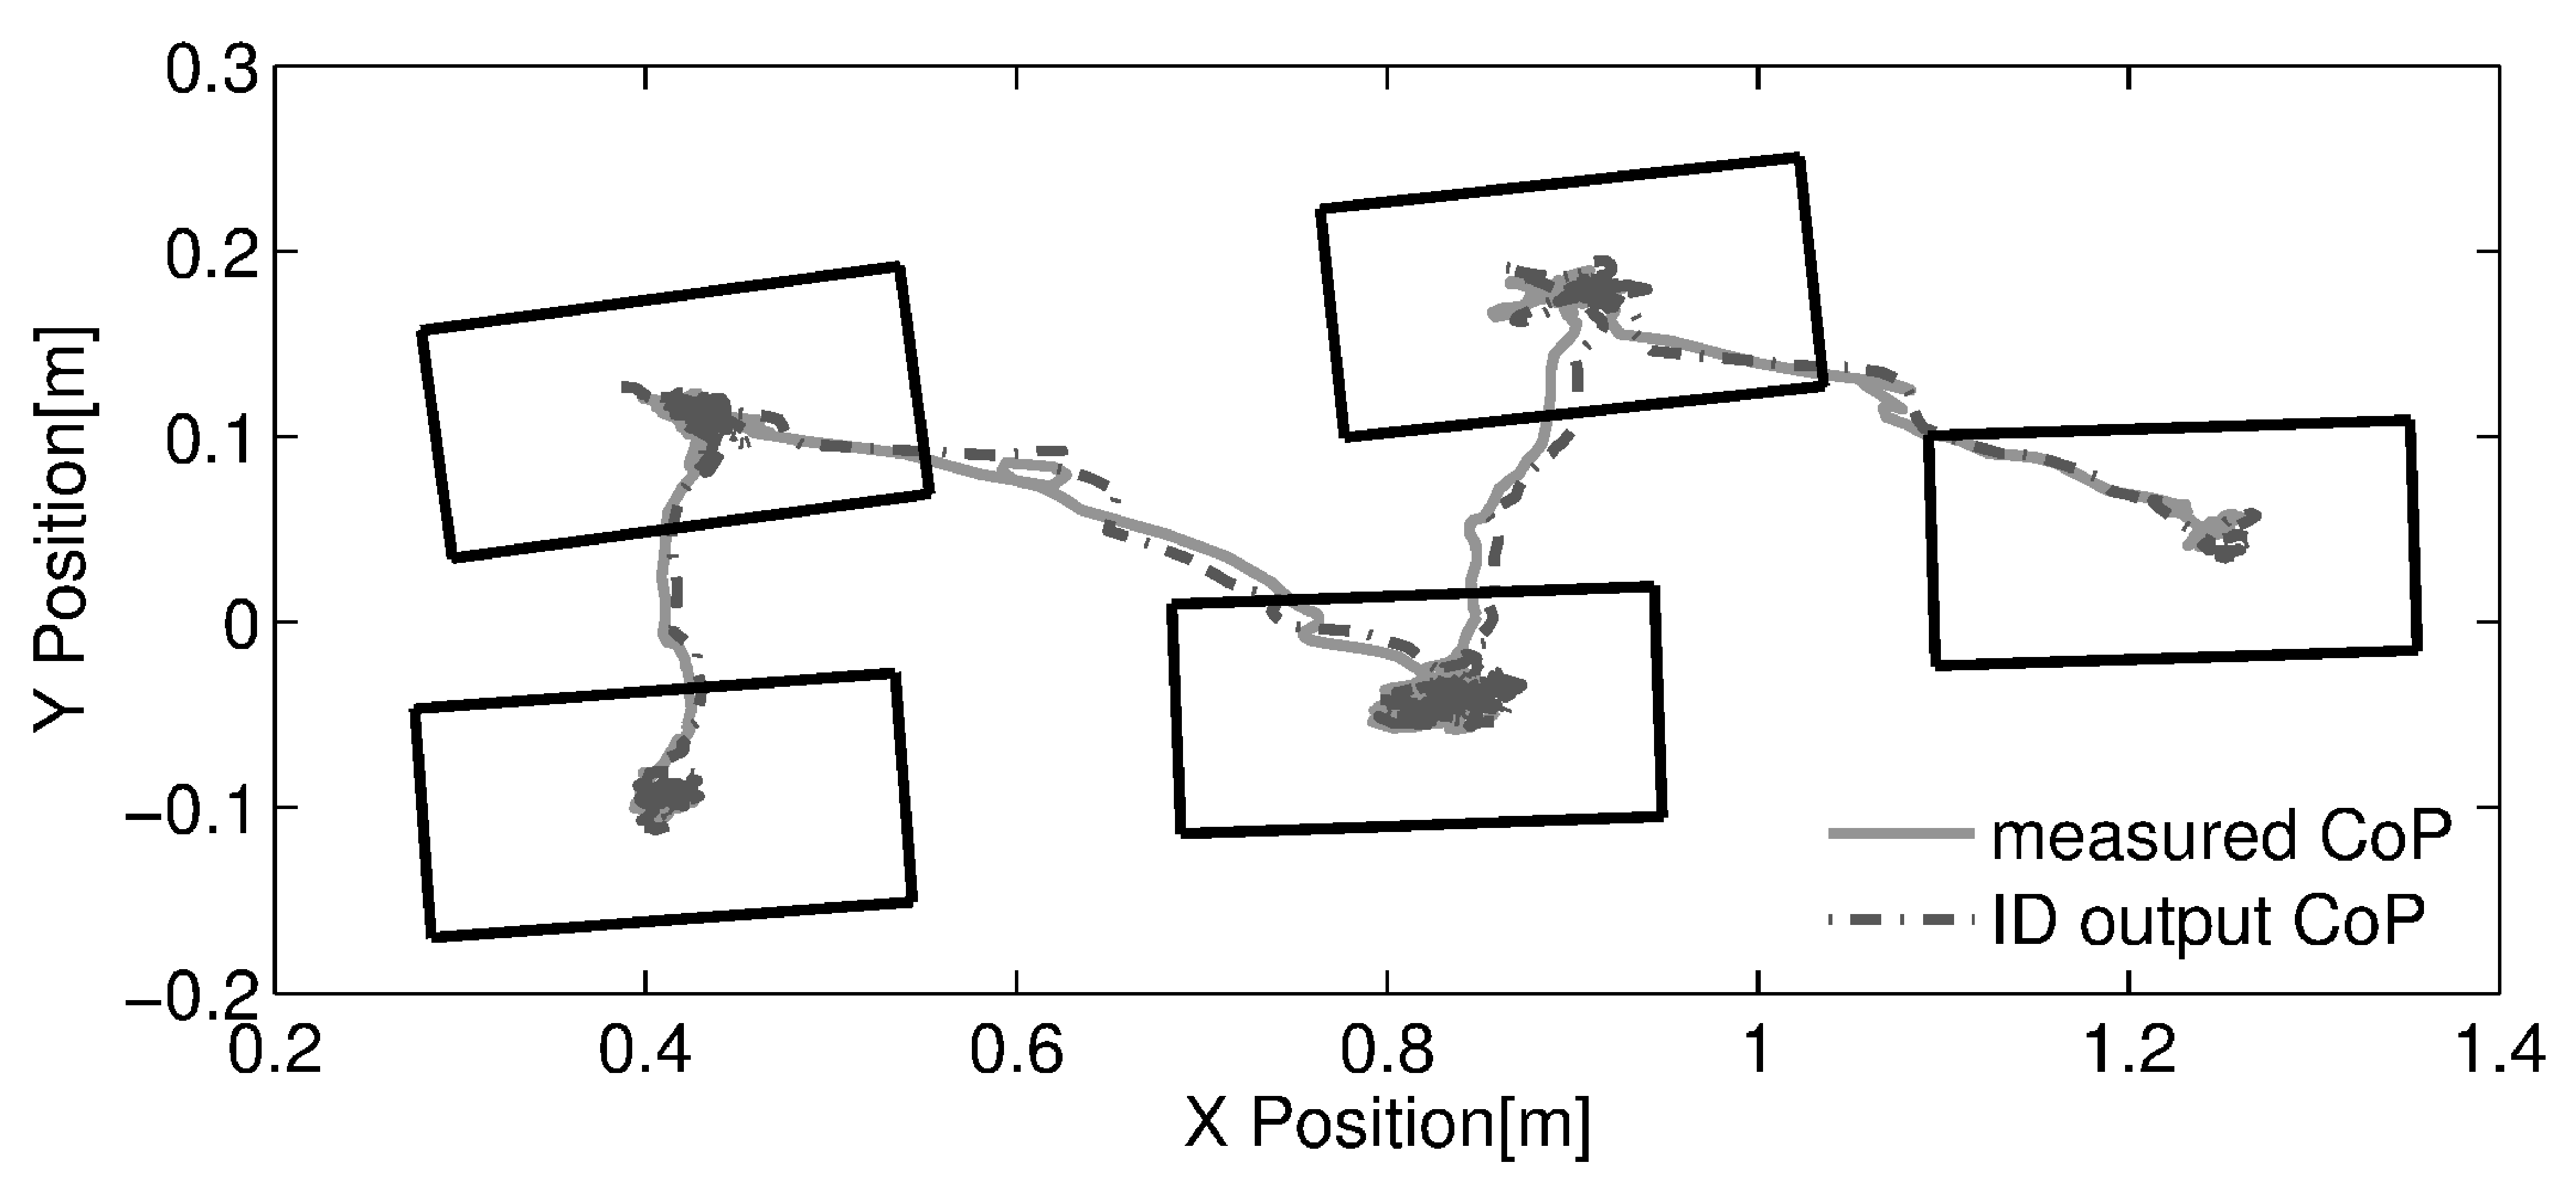
\includegraphics[width=0.9\textwidth]{images/cop_gray.eps} 
    %\subfigure[Root position in Z axis]
    %  {\includegraphics[width=0.45\textwidth]{images/atlas_z.png} \label{subfig:atlas_pelv_z}}
    \caption{
      This plot shows CoP tracking when Atlas was stepping up tilted cinder blocks.}
			%The last row shows pelvis height
      %tracking. Measured root height (state estimator's pelvis position) is 
      %shown in solid blue line. Input to IK is shown in dashed green, and IK's 
      %result is plotted in solid red. 
      %These traces are very similar as well.
      %Cyan and magenta lines represent left 
      %and right foot height. }

    \label{fig:walk_cop} 
  \end{center}
\end{figure}    

\begin{figure}
  \begin{center}
    {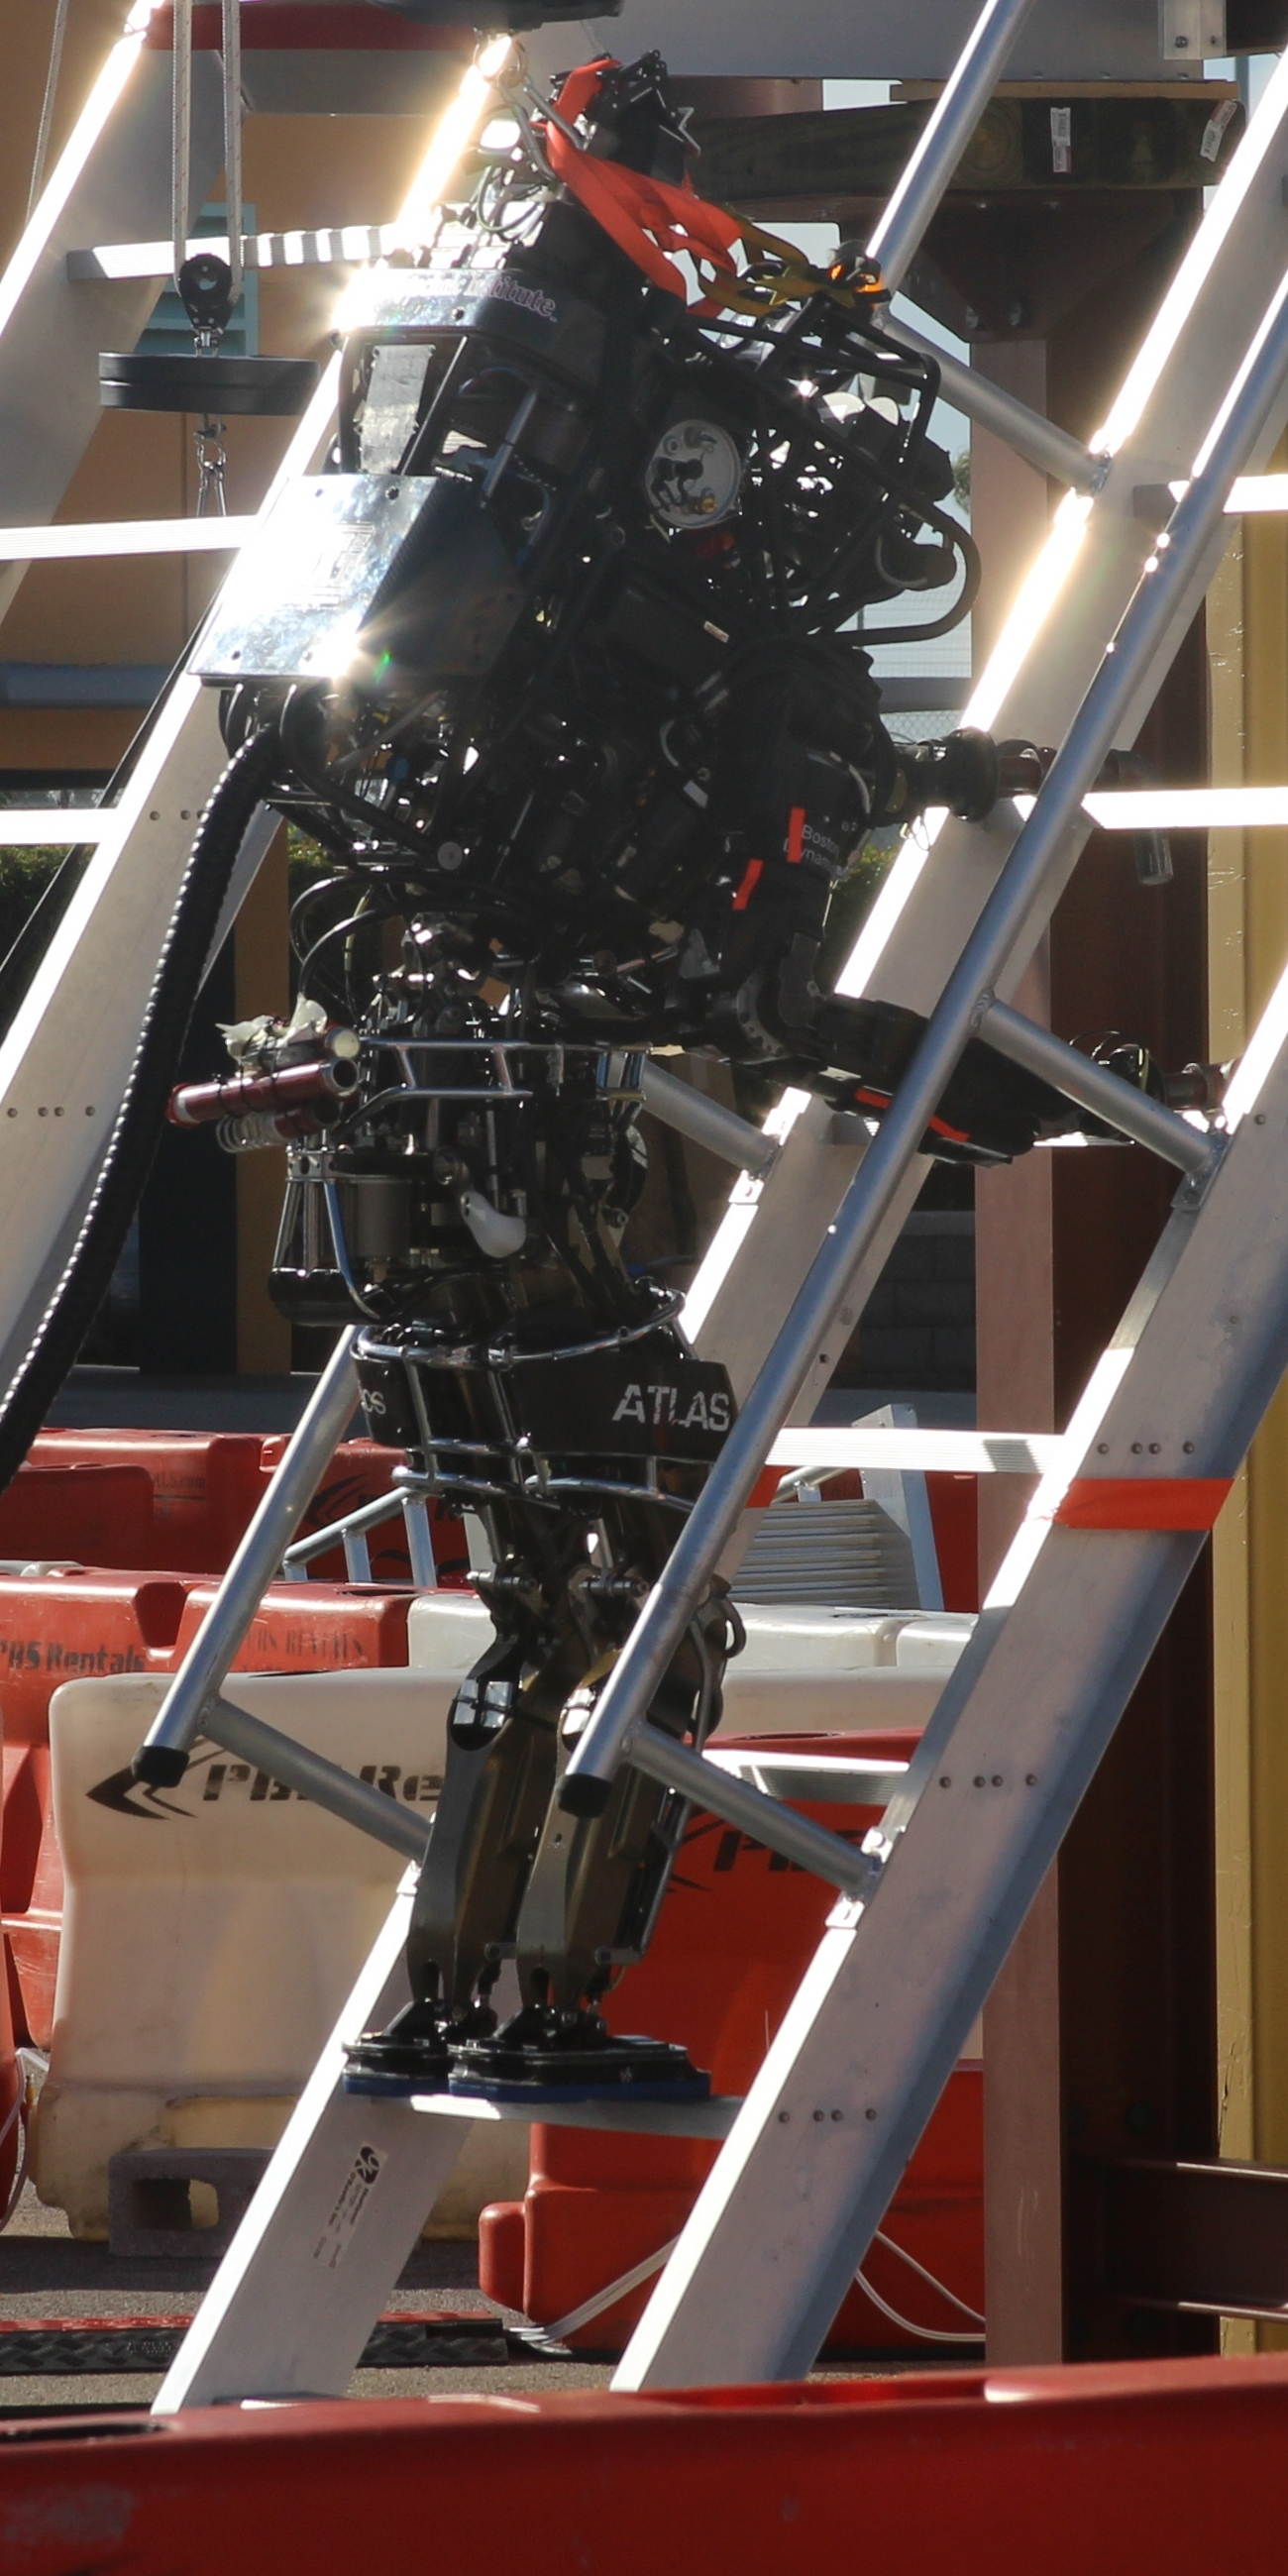
\includegraphics[width=0.9\textwidth]{images/ladder.eps}}
    \caption{
      These photos show the Atlas robot climbing the top half of the same 
      ladder as used in the DRC Trials. 
			The snapshots were taken every 13 seconds. 
			The top row shows re-positioning of the hook hands, 
			and the bottom row shows stepping up one tread. 
			Most of the climbing motions were scripted. 
			After each limb's rough re-positioning, the operator fine adjusted
			its final position with ``nudge'' commands that were small offsets 
			in Cartesian space. 
      }\label{fig:ladder_pic} 
  \end{center}
\end{figure}    

% TODO
% more visible plots
\begin{figure}
  \begin{center}
    \subfigure[Measured limb and CoM trajectories in the $XZ$ plane]
      {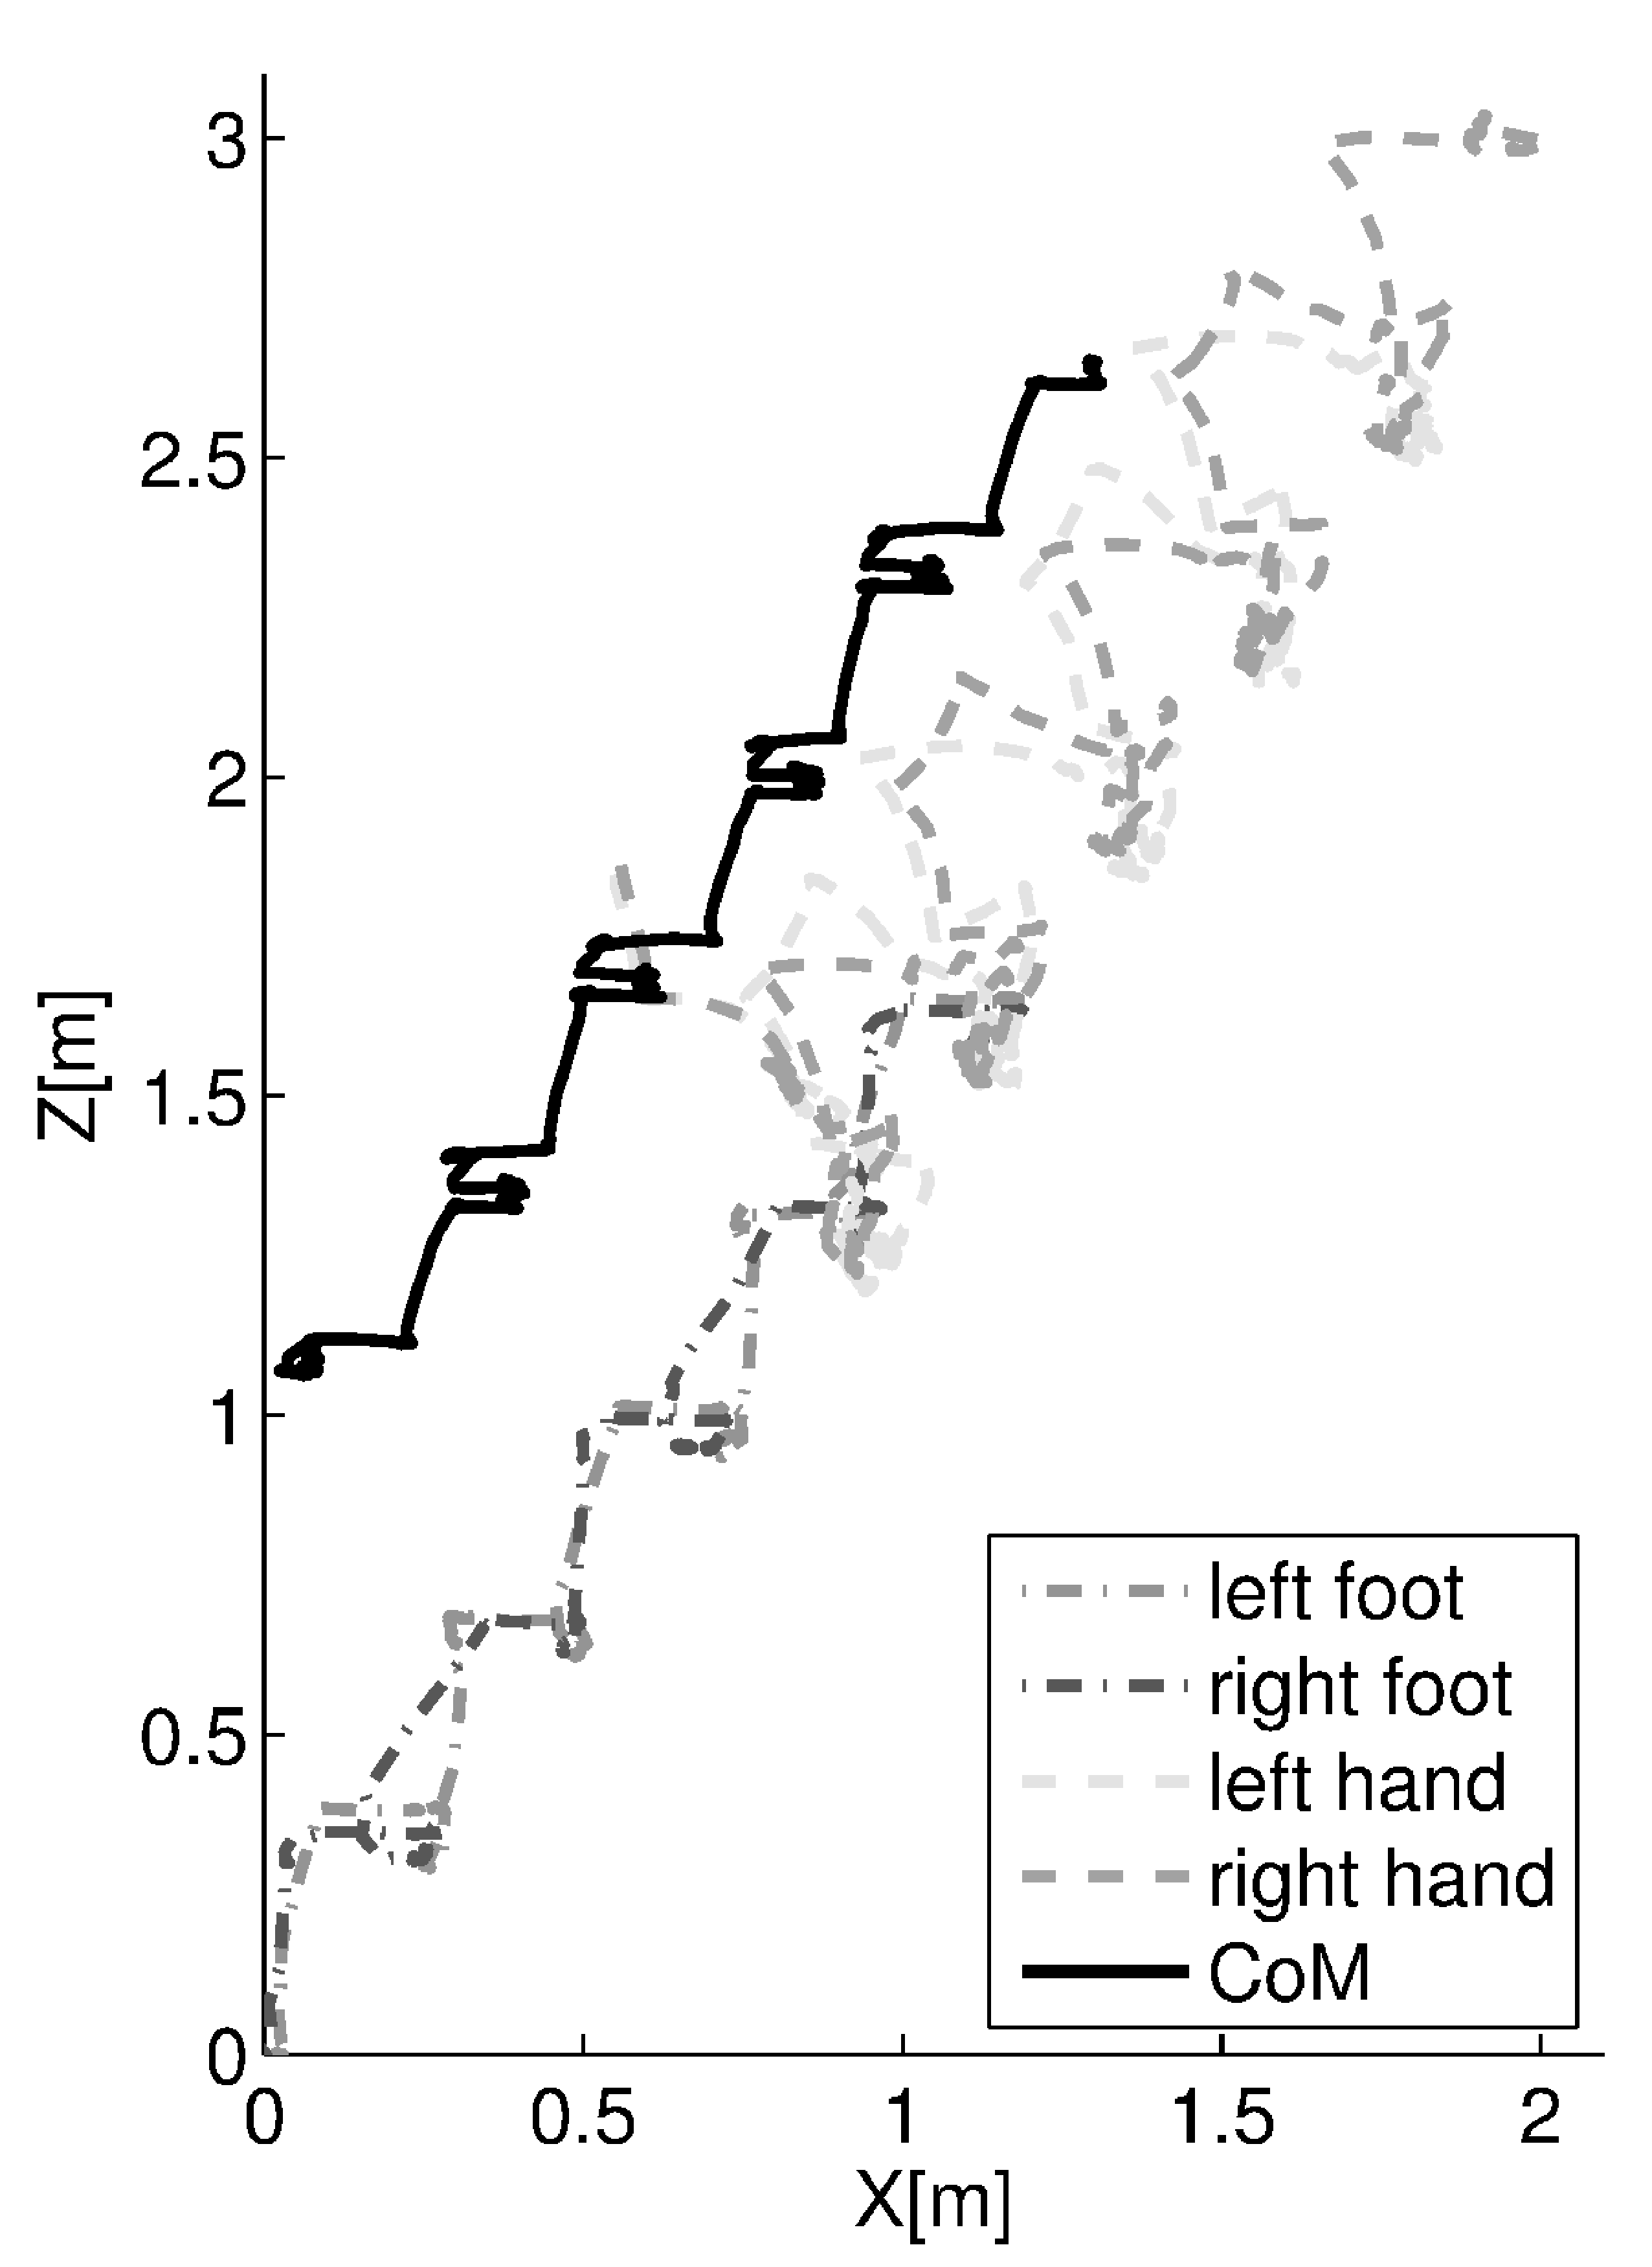
\includegraphics[width=0.45\textwidth]{images/ladder_xz_gray.eps} \label{subfig:ladder_xz}}
    \subfigure[Measured limb and CoM trajectories in the $YZ$ plane]
      {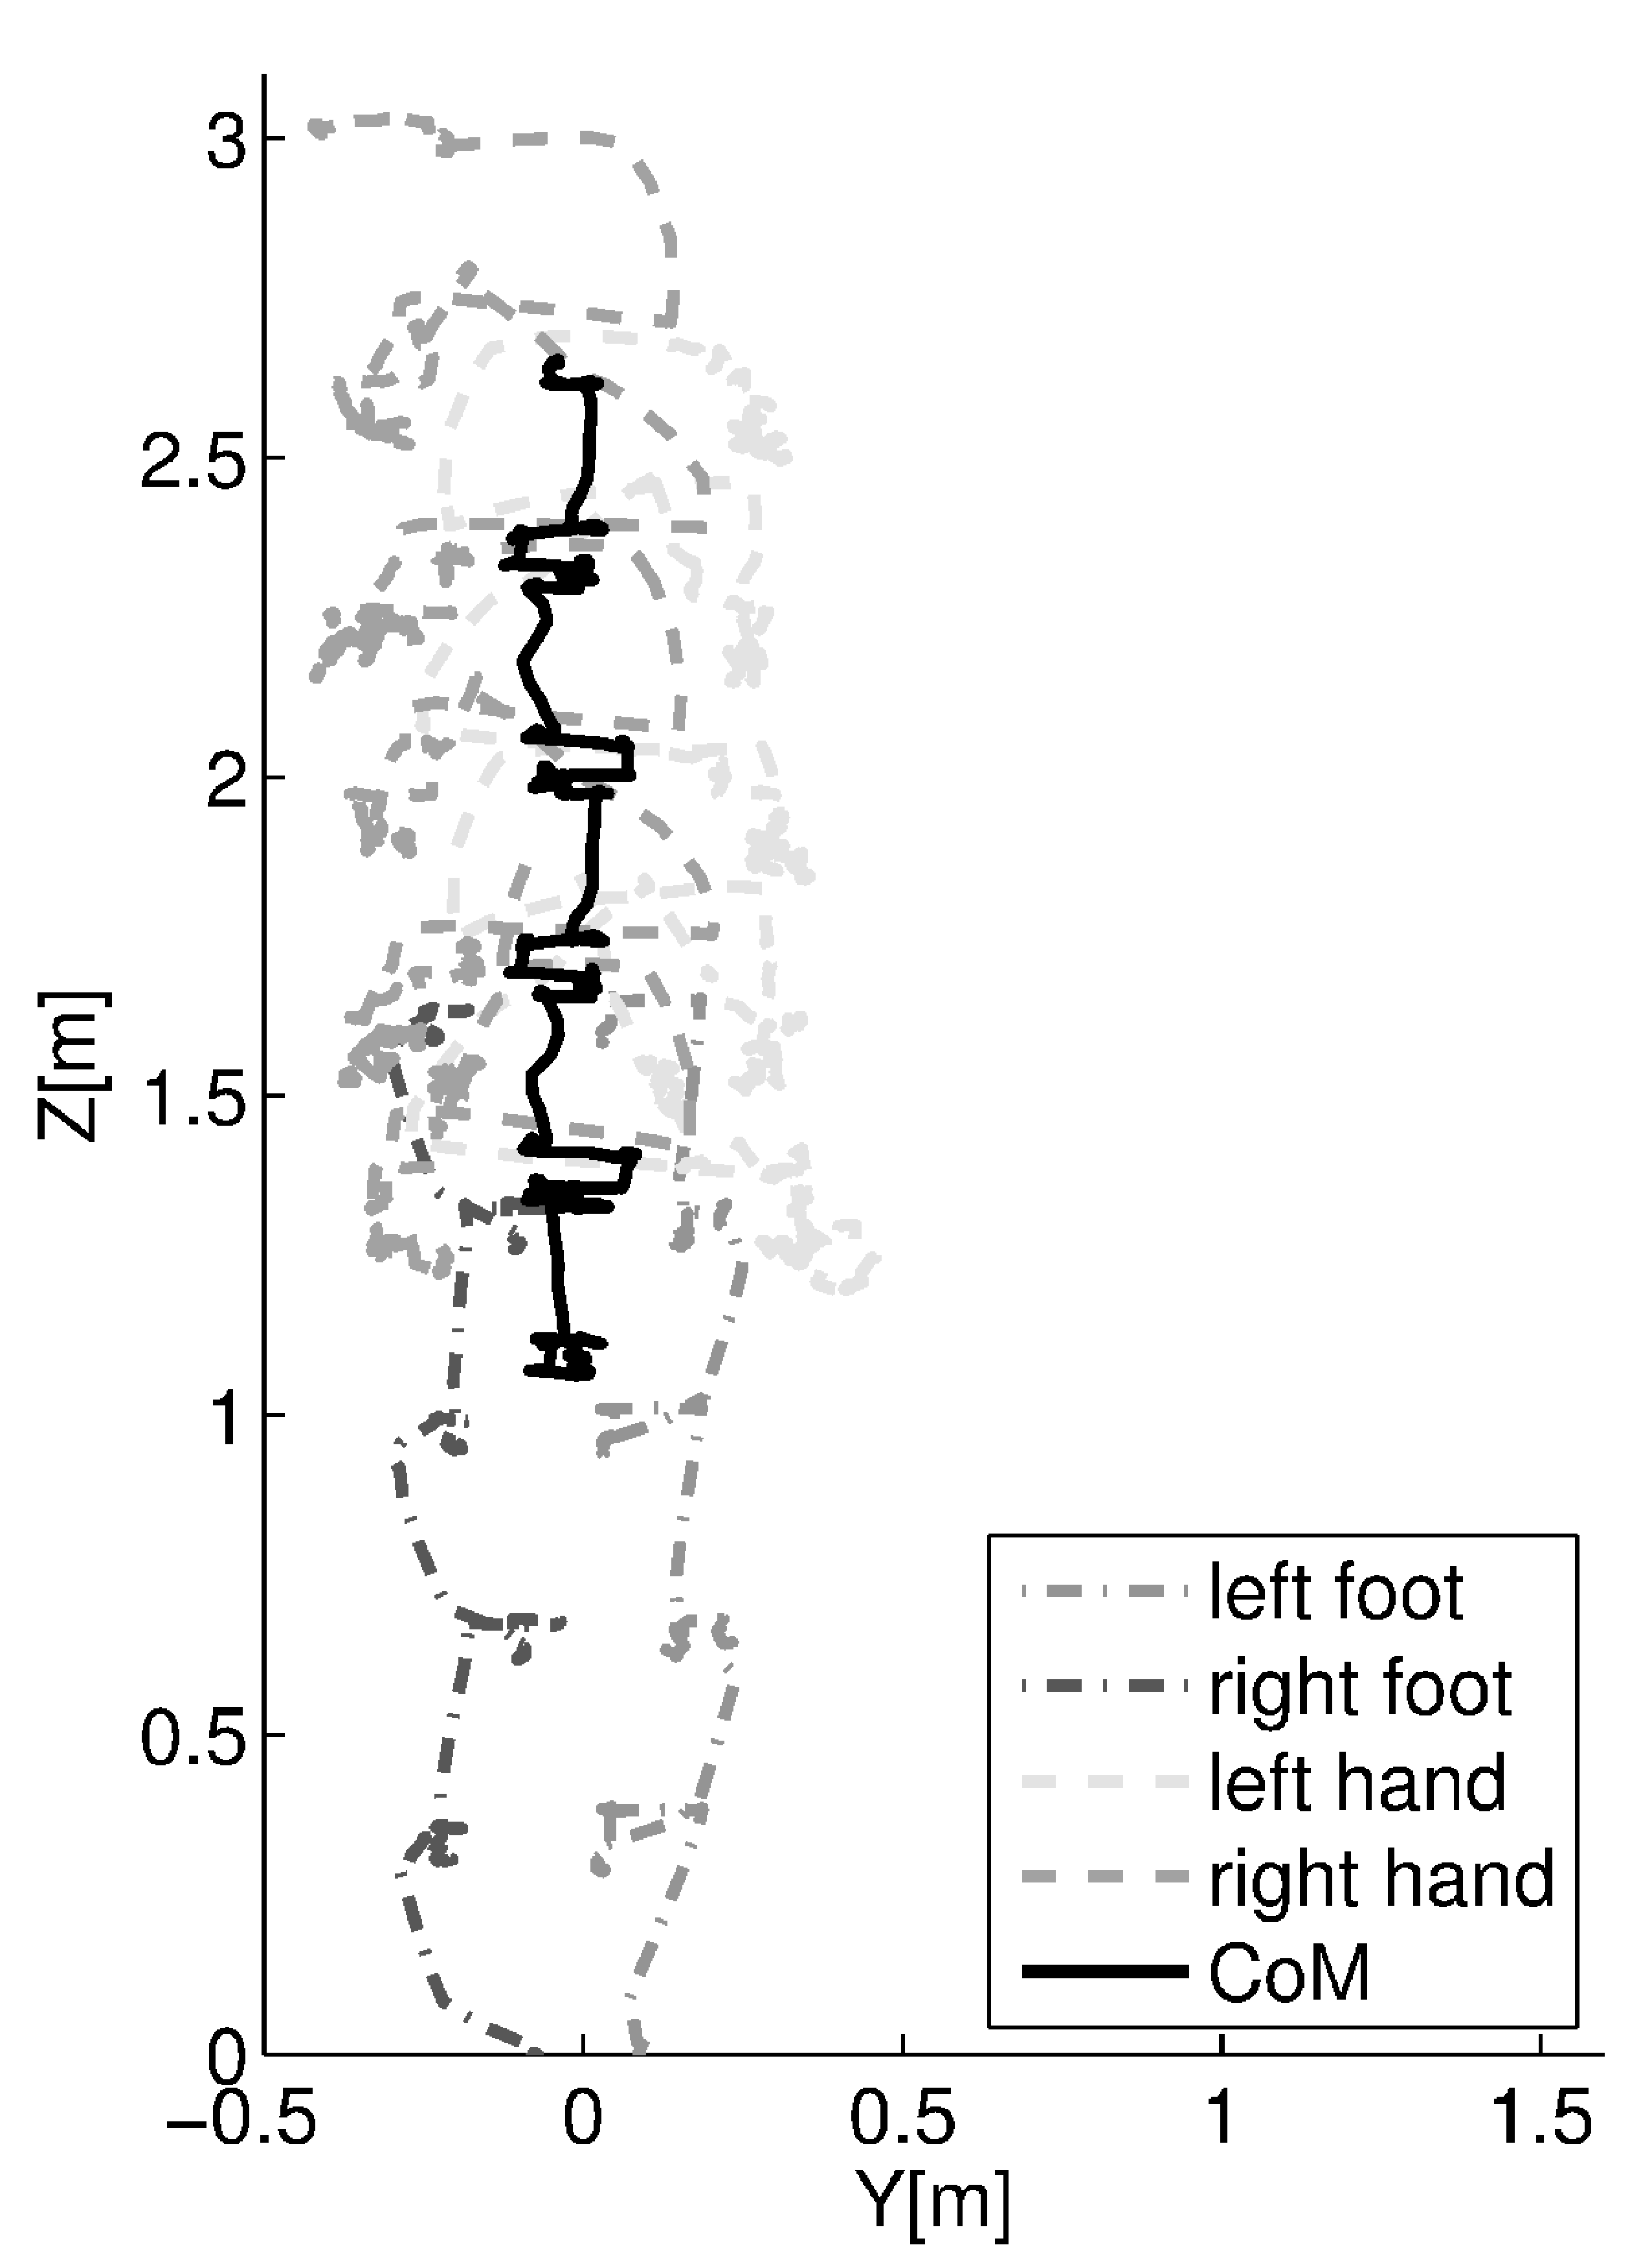
\includegraphics[width=0.45\textwidth]{images/ladder_yz_gray.eps} \label{subfig:ladder_yz}} 
    \caption{
      These two plots show the Atlas robot climbing the first five treads during
      the actual run at the DRC Trials. 
      $X$ axis is the forward direction, $Y$ points to the robot's left, and
      $Z$ points upward. 
      }\label{fig:ladder_data} 
  \end{center}
\end{figure}

\subsection{Full body manipulation}
During full body manipulation, the operator gave commands requesting either 
direct joint angles or target Cartesian poses for one or both hands. 
These commands were used as $x^*_d$ in \eref{eq:id_cart_pd} and \eref{eq:ik_cart_pd}.
We used equality constraints in the IK QP to enforce directly specified joint angles. 
For large Cartesian motions, the new target was connected to the current target
through splines. 
For small motions, we used the ``nudge'' method as described above. 
The controller could also take full body trajectories generated by a motion planner.
\fref{fig:manip} shows snapshots of the Atlas robot executing such a trajectory.

\begin{figure} 
  \begin{center}
    {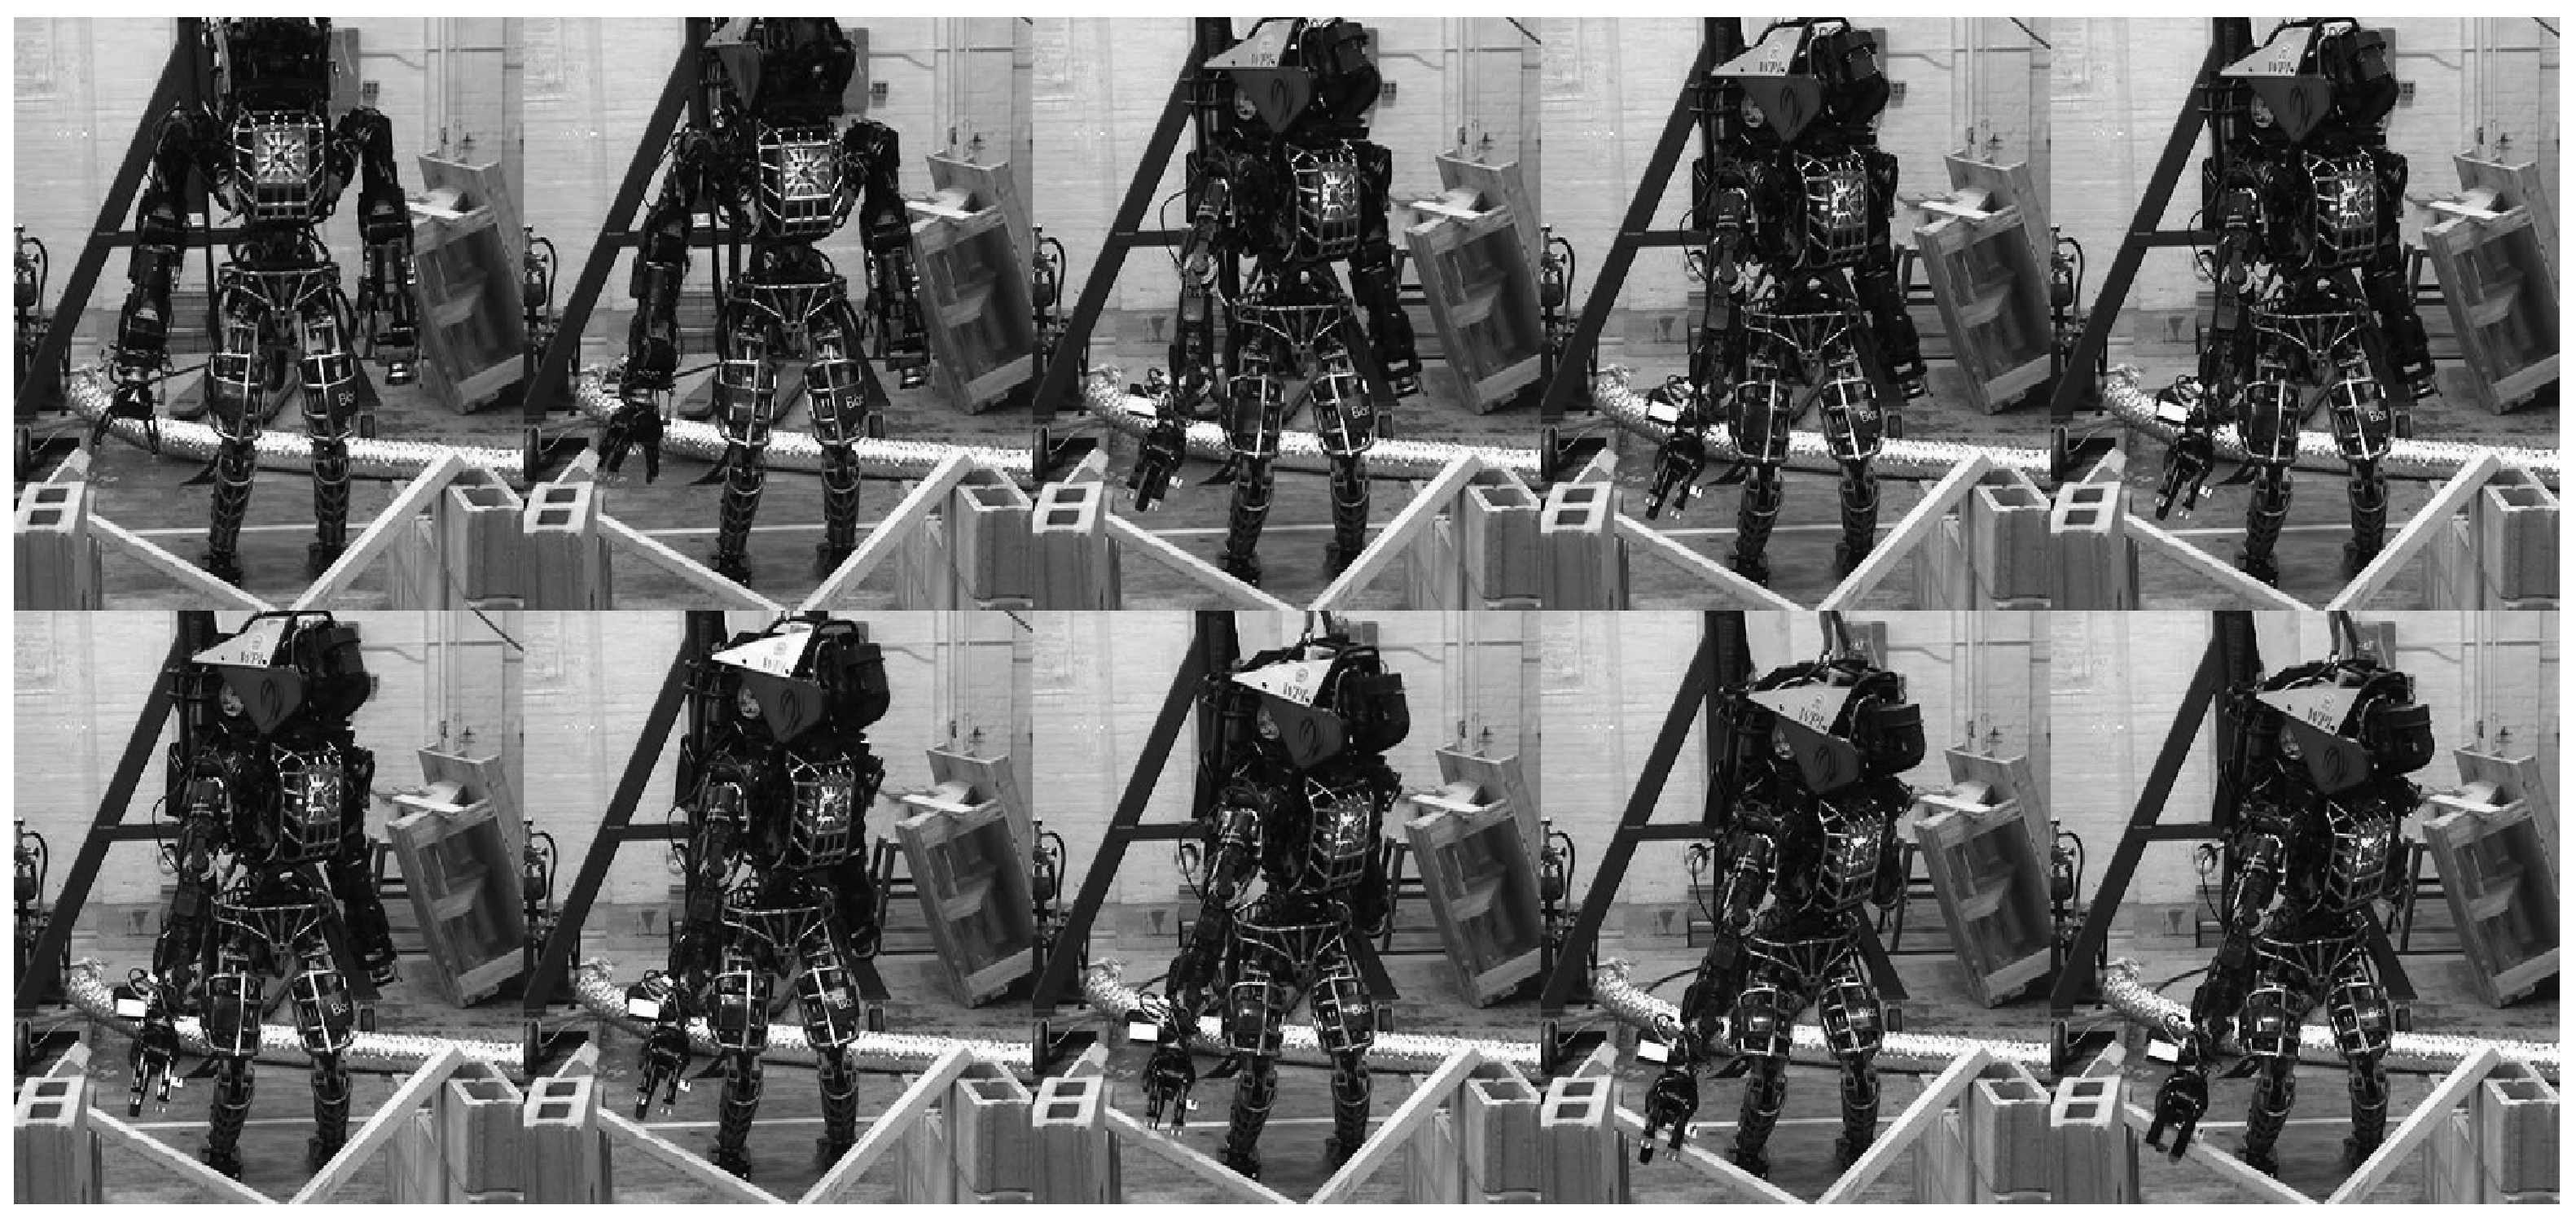
\includegraphics[width=1\textwidth]{images/debris.eps}}
    \caption{The proposed low level controller was applied on the Atlas robot 
      to grab a piece of wood following a planned full body trajectory.}
			\label{fig:manip}
  \end{center}
\end{figure}  
 
A few small changes were made to the basic full body controller:
\subsubsection{No anchoring}
During manipulation, we kept both feet planted and did not take any steps. 
Accordingly, we did not have to worry about the IK position diverging from the 
estimated robot position. 
However, the leaky integrator in \eref{eq:leaky} could result in a failure mode 
characterized by a constant velocity sliding of the foot. 
We called this failure mode a ``chase condition'', and it occurred when 
the contact friction was too low to keep the feet from sliding on its own 
(usually because very little weight was on one of the feet). 
If we constantly updated the IK to the measured position, it could slide farther. 
We therefore disabled this integrator during manipulation.
\label{sec:chase_condition}

\subsubsection{Allowing rotation}
For some tasks, we only cared about the position of the hand, and the 
orientation was unimportant. 
For such cases, we can removed the rotational rows entirely 
in \eref{eq:id_cart} and \eref{eq:ik_cart}. 
For some tasks, we could allow free rotation around one vector, but not 
otherwise. 
For example, while drilling through a wall, the robot can freely rotate the 
drill around the drilling axis, but must maintain its position and keep that 
axis normal to the wall. 
Allowing the controller the freedom to rotate around one axis can drastically 
increase the available workspace. 
This modification was similar to \eref{eq:cart_rot}. 
The rotation was constructed from a basis of three orthogonal unit vectors including 
the desired free-to-rotate-about axis, and the row that corresponded to the 
rotation axis was dropped. 

\subsection{Ladder climbing}
The underlying controller for ladder climbing was similar to that used for 
manipulation, but the majority of the motion was scripted ahead of time with 
only the final placement of the hands and feet controlled by the operator. 
\fref{fig:ladder_pic} shows snapshots of a complete cycle of the Atlas robot
climbing the ladder. 
CoM and limb trajectories from the actual run during the DRC Trials are 
plotted in \fref{fig:ladder_data}. 
Hand or foot was automatically moved to approximately the desired position by 
placing it relative to the other hand or foot. 
Then, the operator precisely placed the limb with 1$cm$ increments using 
``nudge'' commands. 
The correct vertical height was found automatically, using force sensors to 
detect contact for the feet and position sensing when contact was
known to have already occurred for the hands.

Once on the steps, only the toes of the feet were supported, so we adjusted
the CoP constraint accordingly in \eref{eq:id_cop_con}. 
Having all of the weight on the toes made the robot vulnerable to rotational
slipping, causing unexpected yaw rotations.
After such slip occurred, we had to inform the IK controller. 
This issue was analogous the root position divergence problem in the walking
case, but for orientation instead.
In order to correctly place the hands on the next rung to recover from such 
rotations, we periodically rotated the IK solution such that the feet were
aligned with the measured feet orientations. 
The robot would then reorient its upper body towards the ladder and correctly 
reach targets in the real world.  
It would have been preferable to update the orientation continuously, but 
periodic updates were easier from a software engineering perspective.  
Additionally, periodic updates were less susceptible to the ``chase condition''
problem described in \sref{sec:chase_condition}. 
This reorienting served a similar purpose to \eref{eq:leaky}, but for 
rotation instead of translation. 
To avoid chase conditions, this modification was disabled if there was no 
significant (about 20\%) weight on the foot.

\subsubsection{Elbow management}
We climbed the ladder by placing the hands (hooks made from pipes) on the steps.
The robot's shoulders were nearly as wide as the railings, so the necessity of 
shifting weight from side to side resulted in a significant danger of bumping 
the arms on the railings. 
We avoided such collisions by estimating the railing location based on the hand
location (based on the assumption that the hand was pushed up against the side
of the rung) and adding inequality constraints to the IK using \eref{eq:ik_cart_ineq}. 
The inequality constraints limited how far outward each elbow could move in the 
lateral direction. 
Additionally, when we wished to intentionally lean on the railing, we provided 
a desired elbow location (in only the lateral direction) with a low weight. 
To prevent the problem from becoming over-constrained by elbow management, we 
used low weights for commanding hand orientation. 
Specifically, we used \eref{eq:cart_rot} to rotate the hand orientation equations
into a basis containing the hand axis, a pitch-like vector, and a yaw-like vector.
We used a very low, but non-linear weight for rotation about the hand axis 
(roll-like), allowing it roll about 45 degrees nearly freely, but preventing it 
from rolling much farther.

\subsubsection{Hand to CoM integration}
Our forward kinematics based on the robot model was inaccurate. 
One result was that if the hands were resting on one rung and the robot stepped
up one step on the ladder, even though the true position of the hands would not
have moved, the measured position would have moved several centimeters. 
If not accounted for, this would push the CoM far from the desired location, 
eventually resulting in failure. 
We therefore introduced an integrator that gradually adjusted the desired position
of both hands in the horizontal plane based on the deviation between the measured 
and desired CoM position similar to \sref{sec:com_int}. 
Essentially, we were using the arms to pull or push the CoM into the desired 
position. 
To avoid unintentionally rotating the robot, this integrator was only active 
while both hands were in contact with the rung. 

\section{Towards faster walking}
\label{sec:new_stuff}
Although ID was helpful for balancing, the walking controller presented in 
\sref{sec:static_walking} was essentially kinematics driven. 
For slow static walking, the controller hardly run into dynamic constraints, 
which allowed us to use a separate IK module to generate desired joint 
position and velocity. 
As we aim for more dynamic behaviors, these kinematic references need to obey
the underlying dynamic constraints. 

Since the DRC trials, we have developed a new controller based on previous 
work \cite{sfeng_online,sfeng_proposal} that is capable of more dynamic walking
for the Atlas robot. 
The new walking controller is able to achieve 1.7$s$ cadence and 0.4$m$
step length as shown in \fref{fig:fast_walking}. 
The new approach consists of a high level trajectory optimizer that generates
reference CoM and swing foot trajectories using the desired footsteps at a low
frequency, and a full body controller that tracks the reference trajectories 
on every control cycle. 
The new walking controller no longer runs a separate IK module. 
Lower body joint level servos consist of only velocity and torque feedback 
loops. 
The desired torque comes straight from the output of ID, and the desired 
velocity is leaky integrated by
\begin{equation}
  \dot{q}_d = \alpha (\dot{q}_d + \ddot{q}_d dt) + (1-\alpha) \dot{q},
	\label{eq:qd_int}
\end{equation} 
where $\dot{q}_d$ is the desired velocity, $\dot{q}$ is the current 
measured velocity, $\ddot{q}_d$ is the acceleration computed by ID, and $\alpha = 0.99$. 
The velocity loop is necessary for swing leg tracking. 
For the upper body, desired joint positions are directly specified.

\begin{figure} 
  \begin{center}
    {\includegraphics[width=1\textwidth]{images/fast_walking.eps}}
    \caption{Atlas walks with 1.7$s$ cadence and 0.4$m$ step length with the
		new walking controller. The snapshots are taken every 0.43$s$.} 
		\label{fig:fast_walking}
  \end{center}
\end{figure}   

\begin{figure} 
  \begin{center}
    {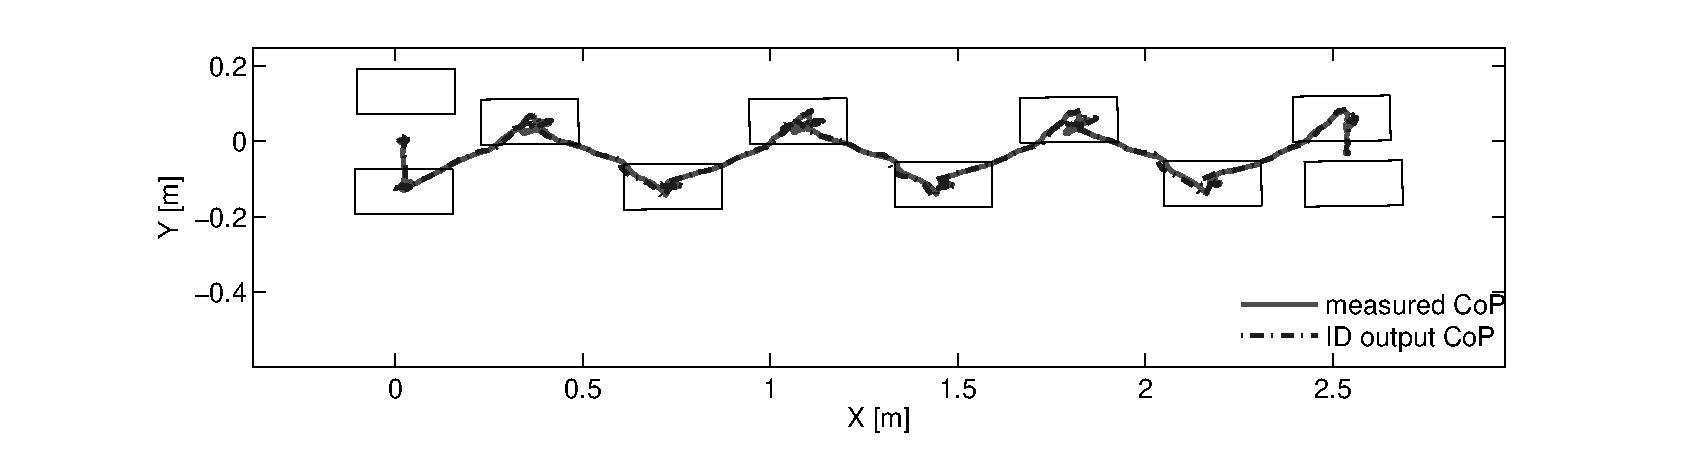
\includegraphics[width=1\textwidth]{images/new_cop.eps}}
    \caption{Atlas walks with 1.7$s$ cadence and 0.4$m$ step length with the
		new walking controller. The snapshots are taken every 0.43$s$.} 
		\label{fig:fast_walking}
  \end{center}
\end{figure}   
 

%%%%%%%%%%%%%%%%%%%%%%%%%%%%%%%%%%%%%%%%%%%%%%%%%%%%%%%%%%%%%%%%%%%%%%%%%%%%%%%%
\section{Discussion and future work}
\label{sec:dis}
During early robot development before the DRC Trials, we found using ID alone is 
insufficient to track the desired motions on the physical robot, especially 
for the swing leg and arms. 
For most joints on the Atlas robot, there is about 10$Nm$ friction, which is
on the same order of torques for tracking joint trajectories when no external
force is applied.
In addition, joint torques are measured by the pressure difference across piston 
chambers, even with an accurate mass model and perfect torque tracking, we still
need to explicitly compensate for friction to achieve good motion tracking.
Hence, some form of kinematics based control is necessary for the lightly loaded
joints, such as those on the swing leg and arms.
Due to the tight time frame for the DRC Trials in December 2013, we introduced
a separate IK pass as a temporary solution, which was suitable for slow and
static tasks such as manipulation and ladder climbing in the DRC Trials. 
For more dynamic behaviors, inconsistency between ID and IK's solutions became 
a major issue. 
Failures occur when IK's solution violates physical dynamic constraints that are 
only properly handled by ID. 
For example, if the desired overall CoM trajectory has accelerations that 
exceed the limits imposed by ground friction, it is physically unachievable. 
However, IK is unaware of such constraints, and it will keep tracking the 
unrealistic desired trajectory. 
Our recent effort towards faster walking demands kinematic references that are 
compatible with the underlying dynamic constraints. 
In the new walking controller, joint accelerations computed by ID are 
integrated into velocities and used as references in the joint level servos. 
We are able to achieve much faster walking speed compared with the previous 
approach that relied on a separate IK module. 

For the DRC Trials, our static approached allowed us to use various integrators to 
compensate for modeling errors easily. 
Being slow also mitigated the effects of all kinds of delays in the system. 
In the current fast walking controller development, we are exploring ways to 
directly compensate CoP tracking delays in the simple point mass model we use 
for CoM trajectory generation. 
We are experimenting with explicitly accounting for torque delays in our ID
formulation as well.  
CoM level modeling errors have been estimated based on LIPM 
dynamics \cite{benx_proposal}, and compensated as an external perturbation 
force acting at the CoM \cite{sfeng_proposal} in the full body controller.
The high level controller also needs to rapidly re-optimize footstep timing and
location in a receding horizon fashion to handle large external perturbations. 
The current low level controllers are optimizing greedily for the current 
time step. 
Including a value function \cite{scott_qp} that captures the future cost is 
also desirable. 

We hope to increase the overall performance with better models in the near future. 
All the leg joint level sensing on the Atlas robot such as position, velocity 
(numerically differentiated from position) and torque are pre-transmission. 
This hardware design choice alleviates jitter in the low level joint control, 
but introduces problems for forward kinematics and torque control. 
Friction and stiction forces that are unaccounted for degrade performance of torque control. 
Better state estimation technology needs to be developed for more accurate 
kinematic tracking and force control. 


%%%%%%%%%%%%%%%%%%%%%%%%%%%%%%%%%%%%%%%%%%%%%%%%%%%%%%%%%%%%%%%%%%%%%%%%%%%%%%%%

\section{Conclusions}
\label{sec:conclusion}
We modified previous work to implement the proposed controller on the Atlas 
robot. We had successfully demonstrated our approach on three different challenging 
real life applications, uneven terrain traversal, ladder climbing, and 
manipulation during the DRC Trials in December 2013. 
We were the only Atlas team that was able to climb the ladder reliably.  
Our approach used both inverse dynamics and inverse kinematics in the full body 
controller. 
The inverse dynamics module provided more compliant motion and more robustness 
against external perturbation. 
The inverse kinematics module helped us battle modeling errors and made rapid 
real hardware deployment possible.
The combined low level controller abstracted away the details about the physical 
system and provided mechanisms to realize and trade off among potentially 
conflicting objectives while obeying various constraints. 
For more dynamic behaviors, our recent development favors an unified full body
controller that integrates the accelerations from the ID results to generate 
kinematic references instead of a separate IK module.
On the other hand, for more static tasks such as manipulation, the original 
IK and ID combination is still preferred for more accurate position tracking with
the arms.
 
%%%%%%%%%%%%%%%%%%%%%%%%%%%%%%%%%%%%%%%%%%%%%%%%%%%%%%%%%%%%%%%%%%%%%%%%%%%%%%%%

\section*{Acknowledgement}
This material is based upon work supported in part by the US National Science 
Foundation (ECCS-0824077, and IIS-0964581) and the DARPA M3 and the Robotics 
Challenge programs.
 
\bibliographystyle{ieeetr}

\bibliography{sfeng}

\end{document}


